
%% bare_conf_compsoc.tex
%% V1.4b
%% 2015/08/26
%% by Michael Shell
%% See:
%% http://www.michaelshell.org/
%% for current contact information.
%%
%% This is a skeleton file demonstrating the use of IEEEtran.cls
%% (requires IEEEtran.cls version 1.8b or later) with an IEEE Computer
%% Society conference paper.
%%
%% Support sites:
%% http://www.michaelshell.org/tex/ieeetran/
%% http://www.ctan.org/pkg/ieeetran
%% and
%% http://www.ieee.org/

%%*************************************************************************
%% Legal Notice:
%% This code is offered as-is without any warranty either expressed or
%% implied; without even the implied warranty of MERCHANTABILITY or
%% FITNESS FOR A PARTICULAR PURPOSE! 
%% User assumes all risk.
%% In no event shall the IEEE or any contributor to this code be liable for
%% any damages or losses, including, but not limited to, incidental,
%% consequential, or any other damages, resulting from the use or misuse
%% of any information contained here.
%%
%% All comments are the opinions of their respective authors and are not
%% necessarily endorsed by the IEEE.
%%
%% This work is distributed under the LaTeX Project Public License (LPPL)
%% ( http://www.latex-project.org/ ) version 1.3, and may be freely used,
%% distributed and modified. A copy of the LPPL, version 1.3, is included
%% in the base LaTeX documentation of all distributions of LaTeX released
%% 2003/12/01 or later.
%% Retain all contribution notices and credits.
%% ** Modified files should be clearly indicated as such, including  **
%% ** renaming them and changing author support contact information. **
%%*************************************************************************


% *** Authors should verify (and, if needed, correct) their LaTeX system  ***
% *** with the testflow diagnostic prior to trusting their LaTeX platform ***
% *** with production work. The IEEE's font choices and paper sizes can   ***
% *** trigger bugs that do not appear when using other class files.       ***                          ***
% The testflow support page is at:
% http://www.michaelshell.org/tex/testflow/



\documentclass[conference,compsoc]{IEEEtran}
% Some/most Computer Society conferences require the compsoc mode option,
% but others may want the standard conference format.
%
% If IEEEtran.cls has not been installed into the LaTeX system files,
% manually specify the path to it like:
% \documentclass[conference,compsoc]{../sty/IEEEtran}





% Some very useful LaTeX packages include:
% (uncomment the ones you want to load)


% *** MISC UTILITY PACKAGES ***
%
%\usepackage{ifpdf}
% Heiko Oberdiek's ifpdf.sty is very useful if you need conditional
% compilation based on whether the output is pdf or dvi.
% usage:
% \ifpdf
%   % pdf code
% \else
%   % dvi code
% \fi
% The latest version of ifpdf.sty can be obtained from:
% http://www.ctan.org/pkg/ifpdf
% Also, note that IEEEtran.cls V1.7 and later provides a builtin
% \ifCLASSINFOpdf conditional that works the same way.
% When switching from latex to pdflatex and vice-versa, the compiler may
% have to be run twice to clear warning/error messages.
\usepackage[table,xcdraw]{xcolor}
\usepackage[colorinlistoftodos]{todonotes}
\setuptodonotes{inline}






% *** CITATION PACKAGES ***
%
\ifCLASSOPTIONcompsoc
  % IEEE Computer Society needs nocompress option
  % requires cite.sty v4.0 or later (November 2003)
  \usepackage[nocompress]{cite}
\else
  % normal IEEE
  \usepackage{cite}
\fi
% cite.sty was written by Donald Arseneau
% V1.6 and later of IEEEtran pre-defines the format of the cite.sty package
% \cite{} output to follow that of the IEEE. Loading the cite package will
% result in citation numbers being automatically sorted and properly
% "compressed/ranged". e.g., [1], [9], [2], [7], [5], [6] without using
% cite.sty will become [1], [2], [5]--[7], [9] using cite.sty. cite.sty's
% \cite will automatically add leading space, if needed. Use cite.sty's
% noadjust option (cite.sty V3.8 and later) if you want to turn this off
% such as if a citation ever needs to be enclosed in parenthesis.
% cite.sty is already installed on most LaTeX systems. Be sure and use
% version 5.0 (2009-03-20) and later if using hyperref.sty.
% The latest version can be obtained at:
% http://www.ctan.org/pkg/cite
% The documentation is contained in the cite.sty file itself.
%
% Note that some packages require special options to format as the Computer
% Society requires. In particular, Computer Society  papers do not use
% compressed citation ranges as is done in typical IEEE papers
% (e.g., [1]-[4]). Instead, they list every citation separately in order
% (e.g., [1], [2], [3], [4]). To get the latter we need to load the cite
% package with the nocompress option which is supported by cite.sty v4.0
% and later.





% *** GRAPHICS RELATED PACKAGES ***
%
\ifCLASSINFOpdf
  % \usepackage[pdftex]{graphicx}
  % declare the path(s) where your graphic files are
  % \graphicspath{{../pdf/}{../jpeg/}}
  % and their extensions so you won't have to specify these with
  % every instance of \includegraphicssetuptodonotes
  % \DeclareGraphicsExtensions{.pdf,.jpeg,.png}
\else
  % or other class option (dvipsone, dvipdf, if not using dvips). graphicx
  % will default to the driver specified in the system graphics.cfg if no
  % driver is specified.
  % \usepackage[dvips]{graphicx}
  % declare the path(s) where your graphic files are
  % \graphicspath{{../eps/}}
  % and their extensions so you won't have to specify these with
  % every instance of \includegraphics
  % \DeclareGraphicsExtensions{.eps}
\fi
% graphicx was written by David Carlisle and Sebastian Rahtz. It is
% required if you want graphics, photos, etc. graphicx.sty is already
% installed on most LaTeX systems. The latest version and documentation
% can be obtained at: 
% http://www.ctan.org/pkg/graphicx
% Another good source of documentation is "Using Imported Graphics in
% LaTeX2e" by Keith Reckdahl which can be found at:
% http://www.ctan.org/pkg/epslatex
%
% latex, and pdflatex in dvi mode, support graphics in encapsulated
% postscript (.eps) format. pdflatex in pdf mode supports graphics
% in .pdf, .jpeg, .png and .mps (metapost) formats. Users should ensure
% that all non-photo figures use a vector format (.eps, .pdf, .mps) and
% not a bitmapped formats (.jpeg, .png). The IEEE frowns on bitmapped formats
% which can result in "jaggedy"/blurry rendering of lines and letters as
% well as large increases in file sizes.
%
% You can find documentation about the pdfTeX application at:
% http://www.tug.org/applications/pdftex
\usepackage{subfig}




% *** MATH PACKAGES ***
%
\usepackage{amsmath, amssymb, enumitem}
% A popular package from the American Mathematical Society that provides
% many useful and powerful commands for dealing with mathematics.
%
% Note that the amsmath package sets \interdisplaylinepenalty to 10000
% thus preventing page breaks from occurring within multiline equations. Use:
\interdisplaylinepenalty=2500
% after loading amsmath to restore such page breaks as IEEEtran.cls normally
% does. amsmath.sty is already installed on most LaTeX systems. The latest
% version and documentation can be obtained at:
% http://www.ctan.org/pkg/amsmath





% *** SPECIALIZED LIST PACKAGES ***
%
%\usepackage{algpseudocode}
% algorithmic.sty was written by Peter Williams and Rogerio Brito.
% This package provides an algorithmic environment fo describing algorithms.
% You can use the algorithmic environment in-text or within a figure
% environment to provide for a floating algorithm. Do NOT use the algorithm
% floating environment provided by algorithm.sty (by the same authors) or
% algorithm2e.sty (by Christophe Fiorio) as the IEEE does not use dedicated
% algorithm float types and packages that provide these will not provide
% correct IEEE style captions. The latest version and documentation of
% algorithmic.sty can be obtained at:
% http://www.ctan.org/pkg/algorithms
% Also of interest may be the (relatively newer and more customizable)
% algorithmicx.sty package by Szasz Janos:
% http://www.ctan.org/pkg/algorithmicx




% *** ALIGNMENT PACKAGES ***
%
%\usepackage{array}
% Frank Mittelbach's and David Carlisle's array.sty patches and improves
% the standard LaTeX2e array and tabular environments to provide better
% appearance and additional user controls. As the default LaTeX2e table
% generation code is lacking to the point of almost being broken with
% respect to the quality of the end results, all users are strongly
% advised to use an enhanced (at the very least that provided by array.sty)
% set of table tools. array.sty is already installed on most systems. The
% latest version and documentation can be obtained at:
% http://www.ctan.org/pkg/array


% IEEEtran contains the IEEEeqnarray family of commands that can be used to
% generate multiline equations as well as matrices, tables, etc., of high
% quality.




% *** SUBFIGURE PACKAGES ***
%\ifCLASSOPTIONcompsoc
%  \usepackage[caption=false,font=footnotesize,labelfont=sf,textfont=sf]{subfig}
%\else
%  \usepackage[caption=false,font=footnotesize]{subfig}
%\fi
% subfig.sty, written by Steven Douglas Cochran, is the modern replacement
% for subfigure.sty, the latter of which is no longer maintained and is
% incompatible with some LaTeX packages including fixltx2e. However,
% subfig.sty requires and automatically loads Axel Sommerfeldt's caption.sty
% which will override IEEEtran.cls' handling of captions and this will result
% in non-IEEE style figure/table captions. To prevent this problem, be sure
% and invoke subfig.sty's "caption=false" package option (available since
% subfig.sty version 1.3, 2005/06/28) as this is will preserve IEEEtran.cls
% handling of captions.
% Note that the Computer Society format requires a sans serif font rather
% than the serif font used in traditional IEEE formatting and thus the need
% to invoke different subfig.sty package options depending on whether
% compsoc mode has been enabled.
%
% The latest version and documentation of subfig.sty can be obtained at:
% http://www.ctan.org/pkg/subfig




% *** FLOAT PACKAGES ***
%
%\usepackage{fixltx2e}
% fixltx2e, the successor to the earlier fix2col.sty, was written by
% Frank Mittelbach and David Carlisle. This package corrects a few problems
% in the LaTeX2e kernel, the most notable of which is that in current
% LaTeX2e releases, the ordering of single and double column floats is not
% guaranteed to be preserved. Thus, an unpatched LaTeX2e can allow a
% single column figure to be placed prior to an earlier double column
% figure.
% Be aware that LaTeX2e kernels dated 2015 and later have fixltx2e.sty's
% corrections already built into the system in which case a warning will
% be issued if an attempt is made to load fixltx2e.sty as it is no longer
% needed.
% The latest version and documentation can be found at:
% http://www.ctan.org/pkg/fixltx2e


%\usepackage{stfloats}
% stfloats.sty was written by Sigitas Tolusis. This package gives LaTeX2e
% the ability to do double column floats at the bottom of the page as well
% as the top. (e.g., "\begin{figure*}[!b]" is not normally possible in
% LaTeX2e). It also provides a command:
%\fnbelowfloat
% to enable the placement of footnotes below bottom floats (the standard
% LaTeX2e kernel puts them above bottom floats). This is an invasive package
% which rewrites many portions of the LaTeX2e float routines. It may not work
% with other packages that modify the LaTeX2e float routines. The latest
% version and documentation can be obtained at:
% http://www.ctan.org/pkg/stfloats
% Do not use the stfloats baselinefloat ability as the IEEE does not allow
% \baselineskip to stretch. Authors submitting work to the IEEE should note
% that the IEEE rarely uses double column equations and that authors should try
% to avoid such use. Do not be tempted to use the cuted.sty or midfloat.sty
% packages (also by Sigitas Tolusis) as the IEEE does not format its papers in
% such ways.
% Do not attempt to use stfloats with fixltx2e as they are incompatible.
% Instead, use Morten Hogholm'a dblfloatfix which combines the features
% of both fixltx2e and stfloats:
%
% \usepackage{dblfloatfix}
% The latest version can be found at:
% http://www.ctan.org/pkg/dblfloatfix




% *** PDF, URL AND HYPERLINK PACKAGES ***
%
%\usepackage{url}
% url.sty was written by Donald Arseneau. It provides better support for
% handling and breaking URLs. url.sty is already installed on most LaTeX
% systems. The latest version and documentation can be obtained at:
% http://www.ctan.org/pkg/url
% Basically, \url{my_url_here}.




% *** Do not adjust lengths that control margins, column widths, etc. ***
% *** Do not use packages that alter fonts (such as pslatex).         ***
% There should be no need to do such things with IEEEtran.cls V1.6 and later.
% (Unless specifically asked to do so by the journal or conference you plan
% to submit to, of course. )


% correct bad hyphenation here
\hyphenation{op-tical net-works semi-conduc-tor}


\begin{document}
%
% paper title
% Titles are generally capitalized except for words such as a, an, and, as,
% at, but, by, for, in, nor, of, on, or, the, to and up, which are usually
% not capitalized unless they are the first or last word of the title.
% Linebreaks \\ can be used within to get better formatting as desired.
% Do not put math or special symbols in the title.
\title{Towards Reinforcement Learning of Invariants for Model Checking of Interlockings}


% author names and affiliations
% use a multiple column layout for up to three different
% affiliations
\author{\IEEEauthorblockN{Ben Lloyd-Roberts, Phillip James, Michael Edwards}
\IEEEauthorblockA{Department of Computer Science, Swansea University UK\\
Email: \{ben.lloyd-roberts, p.d.james, michael.edwards\}@swansea.ac.uk}}

% conference papers do not typically use \thanks and this command
% is locked out in conference mode. If really needed, such as for
% the acknowledgment of grants, issue a \IEEEoverridecommandlockouts
% after \documentclass

% for over three affiliations, or if they all won't fit within the width
% of the page (and note that there is less available width in this regard for
% compsoc conferences compared to traditional conferences), use this
% alternative format:
% 
%\author{\IEEEauthorblockN{Michael Shell\IEEEauthorrefmark{1},
%Homer Simpson\IEEEauthorrefmark{2},
%James Kirk\IEEEauthorrefmark{3}, 
%Montgomery Scott\IEEEauthorrefmark{3} and
%Eldon Tyrell\IEEEauthorrefmark{4}}
%\IEEEauthorblockA{\IEEEauthorrefmark{1}School of Electrical and Computer Engineering\\
%Georgia Institute of Technology,
%Atlanta, Georgia 30332--0250\\ Email: see http://www.michaelshell.org/contact.html}
%\IEEEauthorblockA{\IEEEauthorrefmark{2}Twentieth Century Fox, Springfield, USA\\
%Email: homer@thesimpsons.com}
%\IEEEauthorblockA{\IEEEauthorrefmark{3}Starfleet Academy, San Francisco, California 96678-2391\\
%Telephone: (800) 555--1212, Fax: (888) 555--1212}
%\IEEEauthorblockA{\IEEEauthorrefmark{4}Tyrell Inc., 123 Replicant Street, Los Angeles, California 90210--4321}}

% use for special paper notices
%\IEEEspecialpapernotice{(Invited Paper)}




% make the title area
\listoftodos


\maketitle


% As a general rule, do not put math, special symbols or citations
% in the abstract
\begin{abstract}
The application of formal methods to verify that railway signalling systems operate correctly is well established within academia and is beginning to see real applications. However, there is yet to be a substantial impact within industry due to current approaches often producing false positive results that require lengthy manual analysis. It is accepted that invariants, properties which hold for all states under which a signalling system operates, can help reduce occurences of false positives. However automated deduction of these invariant remains a challenge. In this work we report on using reinforcement learning to explore state spaces of signalling systems and generate a dataset of state spaces from which we envisage invariants could be mined. Our results suggest the viability of reinforcement learning in both maximising state space coverage and estimating the longest loop free path for state spaces. Proximal Policy Optimisation (PPO) demonstrates the most stable learning, particularly in large environments where the optimal behaviour function is most complex. Whereas, distributed, multi-agent algorithms, such as Asynchronous Advantage Actor-Critic (A3C) result in the greatest state coverage.
\end{abstract}

% no keywords


% For peer review papers, you can put extra information on the cover
% page as needed:
% \ifCLASSOPTIONpeerreview
% \begin{center} \bfseries EDICS Category: 3-BBND \end{center}
% \fi
%
% For peerreview papers, this IEEEtran command inserts a page break and
% creates the second title. It will be ignored for other modes.
\IEEEpeerreviewmaketitle



% no \IEEEPARstart
\section{Introduction}


% Builing on existing approaches to model ladder logic dynamics
% Use of LLP semantics to extract its inputs / outputs to model state transitions 
% Provides an interactive environment for software agents (vars comprise the state and inputs the means to move between them)
% RL provides a sensible inerface for learning patterns over finite graph structures where software agents have autonomy in how they choose to interact with the model, based on a rather simplistic reward scheme and reset logic
% Probabilistic methods won't provide guarantees of completeness but may be able to provide useful heuristics for more comprehensive verification approaches
% Our aim is to incentivise agents to explore long sequences of novel states for state coverage maximisation.
% Motivation for this is two-fold:
% (1) Invariants should hold for substanital subregions or entirety of LLP's reachable state space, therfore agents should try to observe as many unique states / transitions as possible. (they may also hold for unreachable states but we're not interested in them)
% (2) Agent behaviour molded by reward scheme (and some other optional variables) and this must reflect our coverage objective - agents must be rewarded for discovering new states and penalised for state loops (they've potential to get stuck in subregions otherwise and will soley rely on any explorative parameters during training).
% Exploration phase then automatically generates a dataset of state sequences (known as trajectories) from which we hope to mine invariant properties.


Model checking is a formal verification technique stemming from the need to systematically
check whether certain properties hold for different configurations (states) of a given system.
Given a transition system $T$ and a formula (or property) $F$, model checking attempts to verify through refutation that $s \vdash F$ for every system state $s \in T$, such that $T \vdash F$. 

The application of model checking in order to verify railway interlockings is well established within
academia and is beginning to see real applications in industry. As early as 1995, Groote
et al. ~\cite{groote1995safety} applied formal methods to verify an interlocking for controlling the Hoorn-Kersenbooger railway station. Newer approaches to interlocking verification have also been proposed in recent
years ~\cite{fantechi2012some, ferrari2011model, haxthausen2008modelling}. This includes work by Linh et al.~\cite{vu2014formal} which explores the verification
of interlockings written in a similar language to Ladder Logic using SAT-based model
checking. In spite of this, such approaches still lack widespread use within the Rail industry. 

In particular, one of the limitations of such model checking solutions is that verification can fail due to over approximation, typically when using techniques such as inductive verification~\cite{4639322}. Inductive verification fails to consider whether system states which violate a given property are indeed reachable by the system from a defined initial configuration. These false positive  often require manual inspection. One solution is to introduce so-called invariants to suppress false positives~\cite{1688959}. Invariants are properties that hold for sub-regions of the state space. The aim is to introduce invariants that help bound the region of reachable states when model checking. However generating sufficiently strong invariants automatically is complex~\cite{4723646}. 

In this work we take first steps towards using machine learning to generate invariants by providing a first formal mapping of interlocking based state spaces to a reinforcement learning (RL) environment. We then explore how such state spaces can be generated in a controlled manner to test the scalability of our approach on environments where the number of reachable states is known. Finally we provide an analysis of how various reinforcement learning algorithms can be used to effectively explore state spaces in terms of their coverage. We see this as a first step towards mining invariants from such state spaces as this approach would indeed require reasonable coverage. Finally we reflect upon future works in directing our approach to improve exploration and learn invariants from a dataset of state sequences generated by our RL agents. 


\section{Preliminaries}\label{sec:preliminaries}
We now briefly discuss  model checking of railway interlockings and reinforcement learning. For further details we refer the reader to~\cite{kanso2009automated, james2013verification} and \cite{mnih2013playing,schulman2017proximal,mnih2016asynchronous} respectively.

\subsection{Ladder Logic \& Interlockings}\label{sec:ladder_logic}
Interlockings serve as a filter or ‘safety layer’ between inputs from railway operators, such as route setting requests, ensuring proposed changes to the current railway state avoid safety conflicts. As a vital part of any railway signalling system, interlockings are critical systems regarded with the highest safety integrity level
(SIL4) according to the CENELEC 50128 standard. 

Ladder logic is a graphical language widely used to program Programmable Logic Controllers\cite{IECstandard} and in particular the Siemens interlocking systems we consider in this work. From an abstract perspective, ladder logic diagrams can be represented as
propositional formulae. Here we follow the definition of James et al~\cite{james2013verification}. A ladder logic rung consists of the following entities.
%(see~\fig{ladderconnectives}).
\emph{Coils}
%are used to
represent boolean values that are stored for later use as output
variables from the program. A coil is always the right most entity
of the rung and its value is computed by executing the rung from left
to right.
\emph{Contacts} are the boolean inputs of a rung,
with \emph{open} and \emph{closed} contacts representing the values
of un-negated and negated variables respectively.  The value of a coil
is calculated when a rung fires, making use of the current set of
inputs -- input variables, previous output variables,
and output variables already computed for this cycle --
following the given connections.  A horizontal connection between
contacts represents logical conjunction and a vertical connection
represents logical disjunction.

A interlocking executes such a program from top-to-bottom over and over, indefinitely.

More formally, following~\cite{james2013verification} a ladder logic program is constructed in terms of disjoint finite sets
$I$ and $C$ of input and output/state variables. We define $C' = \{ c' \, | \, c \in C \}$ to be a set of new variables
in order to denote the output variables computed by the interlocking in the current
cycle.

\textit{Defn 1. Ladder Logic Formulae:}
A ladder logic formula $\psi$ is a propositional formula of the form
$$\psi \equiv ((c'_1 \leftrightarrow \psi_1) \wedge (c'_2 \leftrightarrow
\psi_2) \wedge  \ldots \wedge (c'_n \leftrightarrow \psi_n)$$ 
Where each conjunct represents a rung of the ladder,
such that the following holds for all $i,j\in \{1,\ldots,n\}$:
\begin{itemize}
\item $c'_i \in C'$ (i.e. c' is a coil)
\item $i \neq j \rightarrow c'_i \neq c'_j$ (i.e. coils are unique)
\item $vars(\psi_i) \subseteq I \cup  \{c'_1, \ldots, c'_{i-1} \} \cup \{ c_i, \ldots , c_n \}$ (i.e. the output variable $c_i'$ of  each rung $\psi_i$, may depend on  $\{ c_i, \ldots , c_n \}$ from the previous cycle, 
but not on $c_j$ with $j<i$, due to the nature of the ladder logic implementation,
those values are overridden.)
\end{itemize}
 \todo{Introduce ladder program}

\begin{algorithmic}
	\State (CROSSING$^\prime$  $\leftrightarrow$ (REQ $\land$ $\lnot$ CROSSING), 
	\State REQ$^\prime$  $\leftrightarrow$ (PRESSED $\land \lnot$ REQ), 
	\State TL\_1\_G$^\prime$  $\leftrightarrow$ (($\lnot$ CROSSING$^\prime$) $\land$ ($\lnot$ PRESSED $\lor$ REQ$^\prime$)),
	\State TL\_2\_G$^\prime$  $\leftrightarrow$ (($\lnot$ CROSSING$^\prime$) $\land$ ($\lnot$ PRESSED $\lor$ REQ$^\prime$)), 
	\State TL\_1\_R$^\prime  \leftrightarrow$ CROSSING$^\prime$,
	\State TL\_2\_R$^\prime  \leftrightarrow$ CROSSING$^\prime$,
	\State PL\_1\_G$^\prime  \leftrightarrow$ CROSSING$^\prime$,
	\State PL\_2\_G$^\prime  \leftrightarrow$ CROSSING$^\prime$,
	\State PL\_1\_R$^\prime  \leftrightarrow \lnot$ CROSSING$^\prime$,
	\State PL\_2\_R$^\prime  \leftrightarrow \lnot$ CROSSING$^\prime$, 
	\State AUDIO$^\prime  \leftrightarrow$ CROSSING$^\prime$)
\end{algorithmic}

\subsection{Transition Systems and Model Checking for Ladder Logic}
For this work, we have concentrated on trying to produce invariants for the approaches taken by Kanso et al.~\cite{kanso2009automated} and James et al.~\cite{james2013verification}. Here we include their model of ladder logic based railway interlocking programs as we use this as a basis for defining a learning environment.

Building upon the propositional representation of a ladder logic program given in Section~\ref{sec:ladder_logic}, we can define, following~\cite{james2013verification}, the semantics of a ladder logic program in terms of labelled transition systems.

Let $\{0,1\}$ represent the set of boolean values and let
\begin{align*}
 Val_I  &= \{ \mu_I \, | \, \mu_I : I \to \{0 , 1 \} \}  = \{0,1 \}^I   \\
 Val_C &=  \{ \mu_C \, | \, \mu_C : C \to \{ 0 , 1 \} \} = \{ 0,1 \}^C 
\end{align*}
be the sets of valuations for input and output variables.

The semantics of a ladder logic formula $\psi$ is a function that takes the two current valuations and returns a new
valuation for output variables.
\begin{align*}
 & [ \psi ] : Val_I \times Val_C \to  Val_C \\
 & [ \psi ] ( \mu_I, \mu_C ) = \mu'_C 
\end{align*}
where $\mu'_C$ is computed as follows: the value of each variable $c_i$ is computed using the $i$th rung of the ladder, $\psi_i$, using the valuations $\mu_C$ and $\mu_I$ from the last cycle and the current valuations restricted to those evaluated be fore the current variable. We refer the reader to ~\cite{james2013verification} for full details.

\textit{Defn 2. Ladder Logic Labelled Transition System:}
We define the labelled transition system $LTS(\psi)$ for a ladder logic formula $\psi$ as the tuple $(Val_C,Val_I,\rightarrow, Val_0)$ where
\begin{itemize}
\item $Val_C = \{ \mu_C | \mu_C : C \to \{ 0 , 1 \} \}$ is a set of states.
\item $Val_I = \{ \mu_I | \mu_I : I \to \{0 , 1 \} \}$ is a set of transition labels.
\item $\rightarrow \; \subseteq Val_C \times Val_I \times Val_c $ is a labelled transition relation, where $\mu_C \xrightarrow{\mu_I} \mu'_C$ iff  $[ \psi ] ( \mu_I , \mu_C) = \mu'_C$.
\item $ Val_0 \subseteq Val_C$ is the set of initial states.

\end{itemize}
%
We write $ s \xrightarrow{t} s'$ for $(s,t,s')\in R$.
A state $s$ is called \emph{reachable} if 
$s_0 \xrightarrow{t_0} s_{1} \xrightarrow{t_1} \ldots 
\xrightarrow{t_{n-1}} s_n$,  
for some states $s_0,\ldots, s_{n} \in Val_C$, and 
labels $t_0, \ldots, t_{n-1} \in Val_I$ such that
$s_0 \in Val_0$.  

Consider Figure~\ref{fig_sim}, which, within one Figure, illustrates multiple models of a simple ladder logic program for controlling a pelican crossing\footnote{Here we omit the ladder logic code and refer the reader to \cite{james2013verification}}\todo{Remove footnote if we're keeping the ladder code in sect \ref{sec:ladder_logic}} as considered by James et al~\cite{james2013verification}. One model highlighted is, as defined, a ladder logic LTS. We can see that states contain Boolean valuations for the ladder logic variables (for the LTS model we note the input variables below the dashed line at the bottom of each state are not included in the state variables). For example state S1 shows that the variable CROSSING is $0$ (i.e. false) in that state. Transitions are labelled with (for our purposes here the blue labels) inputs and their Boolean valuations. For instance the arrow from S1 to S2 is labelled with the input PRESSED$=1$. Finally we can also see one initial state, state S0 (the state with dotted edges), where all variables are set to false.

\subsection{Reinforcement Learning and MDPs}
Reinforcement Learning (RL) is a machine learning paradigm with demonstrably impressive capacity for modelling sequential decision making problems as the optimal control of some incompletely-known Markov Decision Process (MDP)~\cite{sutton2018reinforcement}.

\textit{Defn 3. Markov Decision Process} A finite discounted Markov Decision Process $M$ is a five tuple $(S,\mathcal{A},P_a(s,s^\prime), R_a(s,s^\prime),\gamma)$, where 
\begin{itemize}
	\item $S$, is a finite set of states, known as the observation space or state space, representing the model state at discrete time steps.
	\item $\mathcal{A}$, describes the action space; a set of actions performable at discrete time steps, used to compute new states from the observation space.
	\item $P_a(s,s^\prime) = Pr(s_{t+1} = s^\prime | s_t, a_t)$, describe state transition probabilities; the likelihood of observing state $s_{t+1}$ given action $a_t$ is taken from state $s_t$.
	\item $R_a(s,s^\prime)$ is a reward function feeding a scalar signal, $r$ back to the agent at each time step $t$. 
	\item $\gamma \in [0,1]$ is a discount scalar successively applied at each time step.
\end{itemize}

%This user defined \textit{environment}, $\mathcal{E}$, comprises a set of %unique states $\mathcal{S}$, a set of permitted actions from each state $\mathcal{A}(s)$, a function describing state transitions $f : S \times \mathcal{A} \to S^{\prime}$ and a scalar reward signal $r_t$.

In an RL setting we refer to the MDP as our environment, $\mathcal{E}$ where through simulation, software agents sample actions $a \in \mathcal{A}$, observe changes in states, $s \in S$ and learn to optimise some objective based on rewards, $r$ issued over discrete time steps $t$. Simulation can be continuous, where agents indefinitely interact with the environment until some termination criterion is met, such as reaching some reward threshold. Alternatively tasks may be episodic, where training is conducted over a sequence of episodes, defined by a finite number of time steps. It is implicitly assumed ensuing algorithmic descriptions or problem formulation in this work refers to episodic cases. An agent's trajectory, $\tau = (s_1, a_1, r_1,  s_2, a_2, r_2,...,s_h, a_h, r_h)$, summarises experience accumulated over a single episode or continuous training run. Here, $h$ refers to the horizon; a time step beyond which rewards are no longer considered. Rewards observed from time step $t$ up to some terminal time step $T$, are denoted $G_{t} = \sum_{i=t}^{T}\gamma^{i-t}r_{i}$, and referred to as the return. Discount factor $\gamma \in [0,1]$ downscales rewards over return time steps while future rewards are reduced as the discount exponent $i-t$ increases. This helps prioritise immediate rewards over distant ones and enumerate returns over a potentially infinite horizon. 

Two principle challenges of RL are those of prediction and control. The first refers to approximating the value function used to estimate state values $v(s)$ or state-action values $q(s,a)$, describing the benefit of being in that state. Values are differentiable and updated based on an empirical average, known as the expectation, taken over observed returns, $\mathbb{E}[G_t | S_t = s, A_t = a]$. In other words the expectation over return $G_t$ depends being in state $S_t = s$, having taken action $A_t = a$ during the present time step. Observed returns depend on the action(s) sampled at discrete time steps. The second challenge of control concerns optimising this selection process via the policy $\pi(a|s)$; a probability distribution mapping states to actions most likely to maximise the reward objective. Ultimately an optimal value function will converge to an optimal policy~\cite{melo2008analysis}. In practice to scale with complex environments these functions are parametric and approximated with gradient-based methods, such as stochastic gradient ascent.
 
Determining the reachable state space for ladder programs is often intractable, making the complete MDP model unknown to us without computing transitions for all state-action pairs. Consequently we trial several gradient-based learning algorithms using deep neural network state representations to approximate both value function and policy subject to the reward objective. First a simple Deep Q-Network~\cite{mnih2013playing} is trained on small environments before applying more advanced approaches. Among this family of approximate reinforcement learning algorithms are policy gradient methods~\cite{kakade2001natural}. Such algorithms utilise parametrised policies for control, where $\pi(a|s,\theta) = Pr(A_t=a|S_t=s,\theta_t=\theta)$ describes action selection, without need of value function estimates. Actor-critic methods also approximate a parametric, typically state-value, function $\hat{v}(s,\omega)$ separating learning of action selection from predicting value estimates. Gradient updates are performed with respect to parameter vector $\theta$ and objective function $J(\theta)$. Definitions of $J(\theta$) vary depending on the learning algorithm.  In this work we explore the efficacy of three principle actor-critic algorithms; Proximal Policy Optimisation (PPO)~\cite{schulman2017proximal}, Advantage Actor-Critic (A2C) and its asynchronous counterpart (A3C)~\cite{mnih2016asynchronous} in navigating our set of generated LLPs. We discuss the merits and drawbacks of each approach for our setting in Section~\ref{sec:algorithmic_trends}.

\section{Related Work}
Here we briefly highlight key contributions within related literature, addressing the invariant finding problem for interlocking programs and contemporary RL strategies for environment exploration.

\subsection{Invariant Finding}
\todo{Elaborate on these citations}
From software engineering techniques \cite{case2007automated, bensalem1996powerful} to hybrid methods incorporating machine learning \cite{garg2016learning}, researchers have proposed various approaches to invariant finding with varying degrees of success. 
IC3~\cite{bradley11} is one of the most successful approaches for model checking with invariants. IC3 makes use of of relatively simple SAT problems to incrementally constrain a state space towards only reachable states. In this scenario, IC3 operates only at the Boolean level of the abstract state space, discovering inductive clauses over the abstraction predicates. It has been applied to verification of software~\cite{cimatti12} and indeed, in the context of hardware model checking~\cite{bradley07}. Although we note that this approach contains the state-space relative to a given property for verification. In our work, we aim to explore invariants that can be mined independent of the given property.


\subsection{Exploration in Reinforcement Learning}
Maintaining the desired balance between exploring unobserved state-action pairs for information maximisation and exploiting knowledge of the environment to further improve performance remains a challenge in RL research. Means of improving state exploration has seen particular interest in software or user testing communities. In~\cite{9231552}, Bergdahl et al. apply vanilla PPO in an episodic 3D environment, incentivising state space coverage to automatically identify in-game bugs and exploits. Recently, Cao et al.~\cite{9678703} used a curiosity function based on an empirical count of state-action pairs to maximise traversal of state transitions for specific human-machine interfaces, using vanilla Q-learning with an $\epsilon$-greedy exploration. Similar applications in web application testing~\cite{9402046} simulate user actions to navigate site structures, recalling which state-action pairs the model is most 'uncertain'. State transitions with the greatest uncertainty are then prioritised for exploration when backtracking from state loops. Again, authors use vanilla Q-learning and count-based reward scaling during Q-function updates~\cite{tang2017exploration}. Authors of~\cite{9476756} decompose exploration tasks over large, adaptive and partially observable environments into two sub-problems; adaptive exploration policy for region selection and separate policy for exploitation of an area of interest. Other works~\cite{s21041067} incorporate recurrent networks~\cite{medsker2001recurrent} in policy design, using temporality to recall the performance of past actions and their subsequent consequences according to the reward function. In robotics research~\cite{electronics10222751}, Apuroop et al. apply PPO to control hTrihex robot navigation in procedurally generated environments, achieving near human level performance. Novel training algorithms~\cite{manchanda2019learning} have also been devised to learn combinatorial algorithms over large graph structures comprising billions of nodes. We incorporate trends in the literature such as state-of-the-art learning algorithms sporting the best performance in research tasks and using environment reset logic to discourage early convergence. We detail this approach further in Section \ref{sec:results}.


\section{Mapping Formal Methods to Reinforcement Learning} \label{sec:mapping_fm_to_ml}

Before any attempts toward invariant finding can be made, it is essential our model in the reinforcement learning setting captures the structure of model checking on ladder programs. In this section we introduce a faithful mapping that, given a ladder logic LTS, constructs an MDP model where reinforcement learning can be applied. Similarly, any invariant finding approach will require agents that maximise state space coverage. To explore this, we also introduce an approach for generation of state spaces with known metrics such as number of states and state space depth.

\subsection{Ladder Logic Markov Decision Process}\label{subsect:MDP}
%We now define the finite Markov Decision Process (MDP), or environment $\mathcal{E}$ used to represent the LLP. A Ladder Logic MDP $M(\psi)$ is a five tuple $\langle S,\mathcal{A},P_a(s,s^\prime), R_a(s,s^\prime),\gamma \rangle$, where 
%\begin{itemize}
%	\item $S = V_I \cup V_C$, observation space to represent the MDP state at discrete time steps.
%	\item $\mathcal{A} = V_I$, describes the action space; a set of formally defined actions which change the observation space
%	\item $P_a(s,s^\prime) = Pr(s_{t+1} = s^\prime | s_t, a_t)$, describing the likelihood of observing state $s_{t+1}$ given action $a_t$ taken from state $s_t$
%	\item $R_a(s,s^\prime)$ is a reward function fed back to the agent at each time step
%	\item $\gamma$ is a discount scalar applied to the reward estimates for future time steps.
%\end{itemize}

We now define the finite Markov Decision Process (MDP), or environment $\mathcal{E}$ used to represent the LLP. 
\textit{Defn 4. Ladder Logic Markov Decision Process}
A Ladder Logic MDP $M(\psi) = (S,\mathcal{A},P_a(s,s^\prime), R_a(s,s^\prime),\gamma)$ is a five tuple, where our observation space is the union of program inputs and ladder variables, and:


\begin{itemize}
  \item $S = Val_C \cup Val_I$.
  \item $\mathcal{A} = Val_I$.
  \item $P_a(s,s^\prime) = Pr(s_{t+1} = s^\prime | s_t, a_t)$
  \item $R_a(s,s^\prime)$ is a reward function feeding a scalar signal back to the agent at each time step $t$. 
  \item $\gamma \in [0,1]$ is a discount scalar successively applied at each time step.
\end{itemize}

Here we note that any unique valuation of $Val_C$ under the dynamics of a LLP constitutes a distinct state. Our action space, describes the set of ladder logic inputs used to compute new valuations after program execution. $P_a(s,s^\prime) = Pr(s_{t+1} = s^\prime | s_t, a_t)$, describes the state transition function in terms of probabilities of observing $s_{t+1}$ given action $a_t$ is taken from state $s_t$. As here, more transitions are available than described by the ladder logic program, we use this probability distribution to ensure transitions match those defined by the ladder logic (essentially this will be 1 for transitions dictated by the ladder logic program and 0 for transitions that are not). 

Subsequently as agents build a policy $\pi(s|a,\theta)$ according to $R_a(s,s')$ and state transitions observed under $P_a(s,s^\prime)$, the environment unfolds as a set of reachable states that mirror those of the ladder logic LTS. 


Considering Figure~\ref{fig:state_space}, we observe differences in how agent action selection is represented compared to LTS transition labels. Where PRESSED and ACT\_1 are ladder logic inputs, the indices of an agents action space refer to selecting one of the following valuations: [PRESSED=True, PRESSED=False, ACT\_1=True, ACT\_1=False]. One index may evaluate to True (1) while the remainder are False (0). Following Figure~\ref{fig:state_space}, an agent starting its training episode from initial state $S0$ has four available actions (illustrated in red) and three states reachable, $S1,S2,S4$ within the next time step. Selecting action $[0,1,0,0]$ denotes setting PRESSED=False, observing a `new' state $S1$, and receiving positive reward $+1$, completing the time step. For ladder logic MDP with $N$ actions (LTS transition labels), there are at most $2N$ unique transitions $(s,a,s')$, thus the size of the action space from all states $s \in S$, is also $2N$. 

Finally, our reward function and $\gamma$ can be tuned to modify the learning objective. Aiming to maximise state space coverage we implement a reward scheme which positively rewards novel observations over distinct episodes, deterring loop traversal through episode termination and negative rewards. Consider the example trajectory $\tau$ = (S0, [0,1,0,0], +1, S1, [0,0,1,0], +1, S4, [0,1,0,0], +1, S5, [0,1,0,0], -1, S5). Computing the expected return on the next episode, starting from $S0$ and using observed rewards from the latest trajectory, discounting factor $\gamma = 0.99$ applies accordingly; $G_t = 1 + 0.99(1) + 0.99^{2}(1) = 1 + 0.99 + 0.9801$.  In Section~\ref{sec:results} we discuss these point further.

% . Training episodes spawn agents at some initial state, either with all variables set to 0 or from some randomly sampled state from a set of previous observations. Workers are initialised with separate environment instances to accumulate experience independently. A global set of observations is asynchronously updated by workers periodically to compile shared experiences. Early stopping terminates training if a set number of consecutive model updates do not improvement in terms of coverage or reward. Second, training ends in our artificially generated programs if all reachable states have been observed at least once. To aid exploration, on episode resets we randomly initialise workers in some previously visited state, as demonstrated in~\cite{gordillo2021improving}. 


\subsection{Environment Generation}


Given exhaustive search of large state spaces is often computationally intractable, we have generated a set of ladder programs where the number of reachable states and recurrence reachability diameter are known. This enables us to analyse the performance of our approach against well understood state spaces. Using existing models of ladder logic structures as a base template~\cite{james2013verification}, we derive progressively larger programs by sequentially introducing additional rungs. This way a constrained yet predictable pattern of growth is devised. If $|S(\psi_i)|$ represents the number of reachable states for a program $\psi_i$, a subsequently generated program $\psi_{i+1}$ with one additional rung, has $2|S(\psi_i)|+1$ reachable states. Through a series of training runs on each environment we record the number of states observed by workers to gauge the overall state space coverage. 
The following algorithm modifies the body of a pelican crossing ladder program referenced in~\cite{james2013verification}. For every $i^{th}$ rung introduced to lengthen the base program, we define two additional variables, VAR\_$i$ and ACT\_$i$. This effectively doubles the existing state space, increases the size of each state observation and introduces as increments the size of $\mathcal{A}$ by 2.

\begin{algorithmic}\label{algo:ladder_generation}
	\Procedure{Generate Ladder}{$n\_rungs$, $prog$}
	\State cond $\gets$ ($\lnot$ PRESSED $\land$ $\lnot$CROSSING) $\land$ $\lnot$ REQ)
	\State rung $\gets$ ACT\_1 $\land$ cond
	\State coil $\gets$ VAR\_1 $\leftrightarrow$ rung
	\State $i \gets 1$ 
	\While{$i \leq$ n\_rungs}
	\State $i \gets i+1$
	\State new\_rung $\gets$ ACT\_[i] $\land$ (rung)
	\State new\_coil $\gets$ VAR\_[i] $\leftrightarrow$ (new\_rung)
	\State \textbf{append} new\_coil \textbf{to} $prog$
	\EndWhile
	\EndProcedure
\end{algorithmic}
%Figure \ref{fig:state_space} was generated using the additional rung:
%\begin{align*}
%	VAR\_1 = ACT\_1 \land (\lnot PRESSED) \land \\(\lnot CROSSING) \land (\lnot REQ)
%\end{align*}
Applying the above algorithm with $n\_rungs=0$ produces the complete state space of Figure~\ref{fig:state_space}. For readability and illustration we have obfuscated three states from the original ladder program in Section \ref{sec:ladder_logic}, abstracted as the `Pelican State Space'. Similarly, five states and their connected transitions are abstracted as the `Extended State Space'. \todo{Not sure if the following is already explained} Again, dashed edges between states denote transitions invoked by actions we have introduced while hard lined edges are invoked by the valuations of PRESSED. Transition labels from the LTS are highlighted in blue, while action selection according to the RL agent is shown in red. Results presented in Section~\ref{sec:results} are based on a set of generated programs ranging from $2^{14}$ to $2^{50}$ states, referenced in Table~\ref{tab:a3c_results}.

\begin{figure*}[!t]
\centering
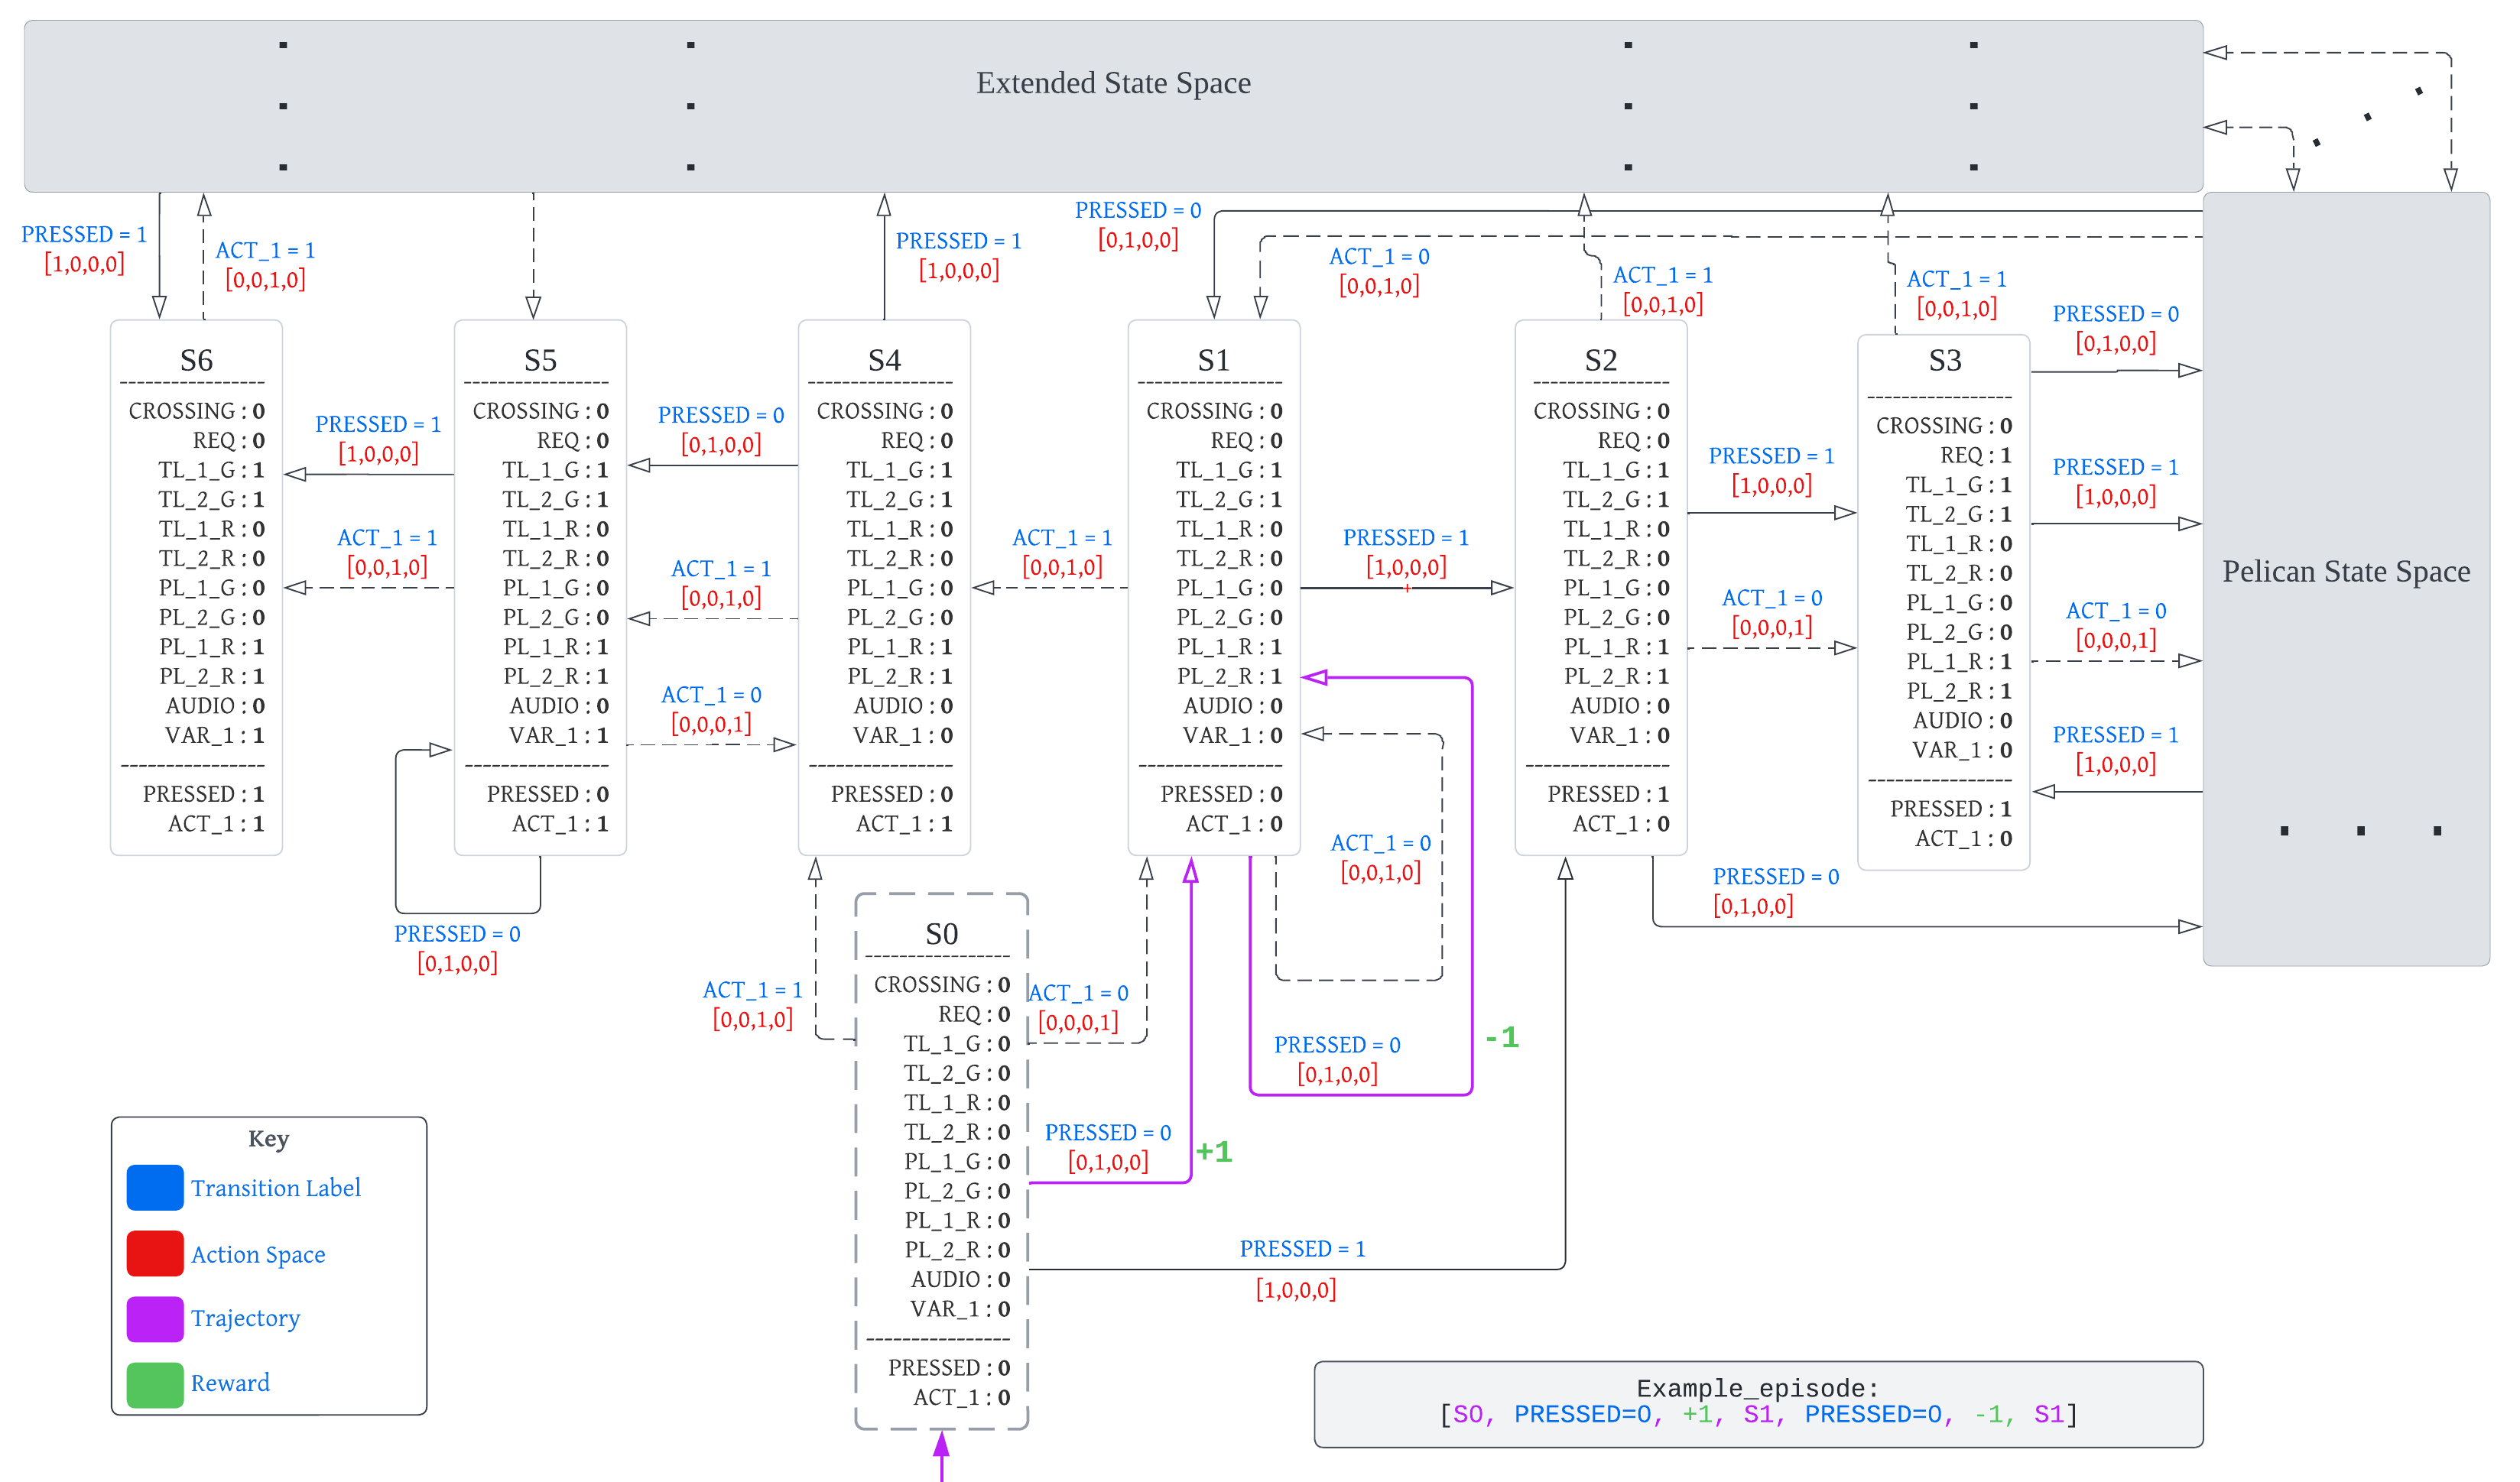
\includegraphics[width=\textwidth]{figs/pelican_states.png}
% where an .eps filename suffix will be assumed under latex, 
% and a .pdf suffix will be assumed for pdflatex; or what has been declared
% via \DeclareGraphicsExtensions.
\caption{Simplified state space representation of generated ladder logic program with one additional input variable ACT\_1 and one output coil VAR\_1.}
\label{fig:state_space}
\end{figure*}

\section{Results}\label{sec:results}
We now present a set of results from applying our approach to a series of generated ladder programs, modelled as learning environments. The following section is divided into three parts, first discussing the merits and drawbacks of the respective learning algorithms. Second, we present results from applying the multi agent A3C algorithm to our full set of generated ladder programs, shown in Table \ref{tab:a3c_results}. Finally we discuss performance differences between single agent implementations of A2C and PPO, as they exhibited divergent learning objectives.


\subsection{Algorithmic Trends}\label{sec:algorithmic_trends}
\todo{Make this coherent} 
Initially to test our model we train a simple DQN agent on a set of generated programs, up to $2^{20}$ theoretic states and 127 reachable. For implementation details regarding The agent often observes complete state coverage within the time taken for the more advanced A2C and PPO algorithms to determine state space depth. DQNs exhibited difficulty scaling well to state space depth learning objective without significant hyperparameter tuning, failing to converge performance on the smallest environments. It is likely using DQN without a prioritised replay buffer~\cite{andrychowicz2017hindsight} leads to poor training sample efficiency when applying network updates. We expect agents exploring ladder program states to rarely observe the greatest depth, meaning episodes resulting in optimal rewards may never be sampled for training. Bootstrapping the action-value function via a target network also introduces an additional challenge in selecting an update interval frequent enough to avoid overestimating state-action values. Similarly, the use of replay memory requires an initial training delay to populate the buffer before Q-Network updates. Setting the gradient step size is likely dependent on the  learnable function complexity, which we'd expect to increase with environment size. The off-policy nature of DQNs constrains network updates with trajectories produced under other, presumably less optimal, policies. Governing the DQN exploration rate explicitly using an $\epsilon$-greedy strategy seems unstable given this could reduce random action exploration with large subregions of an environment unobserved. While DQN demonstrates the potential of RL algorithms in learning policies for prediction and control, they are unlikely to scale sufficiently to interlocking state spaces for the purposes of invariant finding.

Two Actor critic methods, single agent Advantage actor-critic (A2C) and its asynchronous multi-agent counterpart (A3C) are applied to all 19 generated environments. Having several workers and an on-policy learning algorithm removes need of replay memory and any training delay to accumulate sufficient experience. Actor  and critic networks, approximating the behaviour policy and value function, provide better convergence guarantees at the cost of some additional complexity in learned parameters. Paired with randomised reset logic both algorithms accumulate experience faster than conventional DQN, achieving good coverage on a range of medium to large state spaces.  Actor-critic algorithms, while improved by more informed value estimation and policy iteration, they are also susceptible to performance collapse in sufficiently complex environments or over long training periods. Parameter updates have a tendency to push the policy  into an unfamiliar region of policy space from which subsequent updates are unable to recover, potentially `collapsing' the model. Unsurprisingly A3C outperforms the single agent variant and sports the best coverage metric among all policy gradient methods applied. A3C and its results are discussed in depth in Section~\ref{sec:asynch}.

It is for this reason we move to Proximal Policy Optimisation (PPO), to constrain the magnitude of gradient steps during the parameter update. It is our expectation that limiting policy, and potentially value function, updates within a clip range~\cite{schulman2017proximal} or according to KL-divergence between the current and most recent policy~\cite{schulman2017trust}, making the model more resilient to collapse. Trust region methods generally require fewer hyperparameter adjustments being more stable learning strategies. We observe this in Section~\ref{sec:trust_regions}, where PPO demonstrates slow but linear state exploration while appearing to maximise state depth within a known subregion.

\subsection{Asynchronous Exploration}\label{sec:asynch}
\begin{table}[!t]
	\caption{A3C Coverage Metrics}
	\label{tab:a3c_results}
	\centering
	\begin{tabular}{rrrrr}
		\hline
		\multicolumn{3}{c|}{Environment}                                                                                                                                                                     & \multicolumn{2}{c}{Agent}                                \\ \hline
		\multicolumn{1}{c}{\begin{tabular}[c]{@{}c@{}}States\\ (Theoretical)\end{tabular}} & \multicolumn{1}{c}{\begin{tabular}[c]{@{}c@{}}States\\ (Reachable)\end{tabular}} & \multicolumn{1}{c|}{Actions} & \multicolumn{1}{c}{Depth} & \multicolumn{1}{c}{Coverage} \\ \hline
		\rowcolor[HTML]{FFFFFF} 
		$2^{14}$                                                              & 15                                                                               & 2                            & 14                        & 100.0                          \\
		\rowcolor[HTML]{FFFFFF} 
		$2^{16}$                                                              & 31                                                                               & 4                            & 28                        & 100.0                          \\
		\rowcolor[HTML]{FFFFFF} 
		$2^{18}$                                                             & 63                                                                               & 6                            & 48                        & 100.0                          \\
		\rowcolor[HTML]{FFFFFF} 
		$2^{20}$                                                             & 127                                                                              & 8                            & 33                        & 100.0                          \\
		\rowcolor[HTML]{FFFFFF} 
		$2^{22}$                                                              & 255                                                                              & 10                           & 76                        & 100.0                          \\
		\rowcolor[HTML]{FFFFFF} 
		$2^{24}$                                                              & 511                                                                              & 12                           & 49                        & 100.0                          \\
		\rowcolor[HTML]{FFFFFF} 
		$2^{26}$                                                             & 1023                                                                             & 14                           & 306                       & 100.0                          \\
		\rowcolor[HTML]{FFFFFF} 
		$2^{28}$                                                              & 2047                                                                             & 16                           & 538                       & 100.0                          \\
		\rowcolor[HTML]{FFFFFF} 
		$2^{30}$                                                              & 4095                                                                             & 18                           & 1418                      & 99.731                       \\
		\rowcolor[HTML]{FFFFFF} 
		$2^{32}$                                                              & 8191                                                                             & 20                           & 1712                      & 96.532                       \\
		\rowcolor[HTML]{FFFFFF} 
		$2^{34}$                                                              & 16383                                                                            & 22                           & 1498                      & 95.550                       \\
		\rowcolor[HTML]{FFFFFF} 
		$2^{36}$                                                              & 32767                                                                            & 24                           & 2879                      & 84.694                       \\
		\rowcolor[HTML]{FFFFFF} 
		$2^{38}$                                                              & 65535                                                                            & 26                           & 1969                      & 89.071                       \\
		\rowcolor[HTML]{FFFFFF} 
		$2^{40}$                                                              & 131071                                                                           & 28                           & 2692                      & 82.884                       \\
		\rowcolor[HTML]{FFFFFF} 
		$2^{42}$                                                              & 262143                                                                           & 30                           & 1406                      & 76.033                       \\
		\rowcolor[HTML]{FFFFFF} 
		$2^{44}$                                                              & 524287                                                                           & 32                           & 1782                      & 62.137                       \\
		\rowcolor[HTML]{FFFFFF} 
		$2^{46}$                                                              & 1048575                                                                          & 34                           & 1593                      & 64.053                       \\
		\rowcolor[HTML]{FFFFFF} 
		$2^{48}$                                                              & 2097151                                                                          & 36                           & 1598                      & 57.547                       \\
		\rowcolor[HTML]{FFFFFF} 
		$2^{50}$                                                              & 4194303                                                                          & 38                           & 2566                      & 41.483                       \\ \hline
	\end{tabular}
\end{table}

Preliminary results applying the A3C algorithm to a number of generated programs are outlined in Table \ref{tab:a3c_results}. Training was distributed among 32 CPU worker threads. `Actions' referenced in the third column refer to the number of possible assignments over input variables in each ladder program, from every state. Depth, the first agent column, refers to the greatest number of steps taken before repeating observations in the environment, across all workers.

Coverage metrics are expectedly maximised for environments with a small number of reachable states with acceptable levels of coverage for programs with a theoretical size up to $2^{40}$. Interestingly, we observed longer training durations without early stopping occasionally increased coverage beyond a certain threshold. It is possible workers learn an optimal search strategy within a subregion of the state space. Additionally, performance in terms of max depth and states reached increased by approx. $5\%$ when decreasing the total number of episodes from $3 \times 10^{5}$ to $1.5\times10^{5}$ episodes. This may be a product of random episode initialisation spawning workers in more desirable states where stochastic action sampling happened to lead to unfamiliar subregions of the environment.

Performance in terms of cumulative reward which failed to maximise coverage often increased linearly before collapsing to some suboptimal reward. This may be due to tendencies for large network updates to shift the network gradients into a bad local minima, from which performance does not recover within the allotted training duration. The on-policy nature of actor critic means trajectories generated via an old policy are no longer sampled during minibatch updates for the current policy, thus biasing behaviour to the most recent model updates and introducing sample inefficiency. Adding on policy memory strategies\cite{wang2017sample} may help avoid this in future applications

Given the A3C algorithm requires workers to asynchronously update their shared network every $T_{\max}$ steps or on episode termination, larger values for $T_{\max}$ consolidate more information regarding worker trajectories before applying gradient updates to their local network. We found the most significant improvements to performance in terms of coverage metrics and increasing the $k$ bound when introducing workers to larger environments, was lower update frequencies and random start state initialisation. Prior to these adjustments workers, irrespective of their number, seldom covered 80\% of most smaller environments. Similarly, for the largest environment with $2^{50}$ states, coverage improved from 3.2\% to 41.48\%

\subsection{Trust Regions and Reward Shaping} \label{sec:trust_regions}

\begin{figure*}[!t]
\centering
\subfloat[Number of reachable states discovered during five hours of training.]{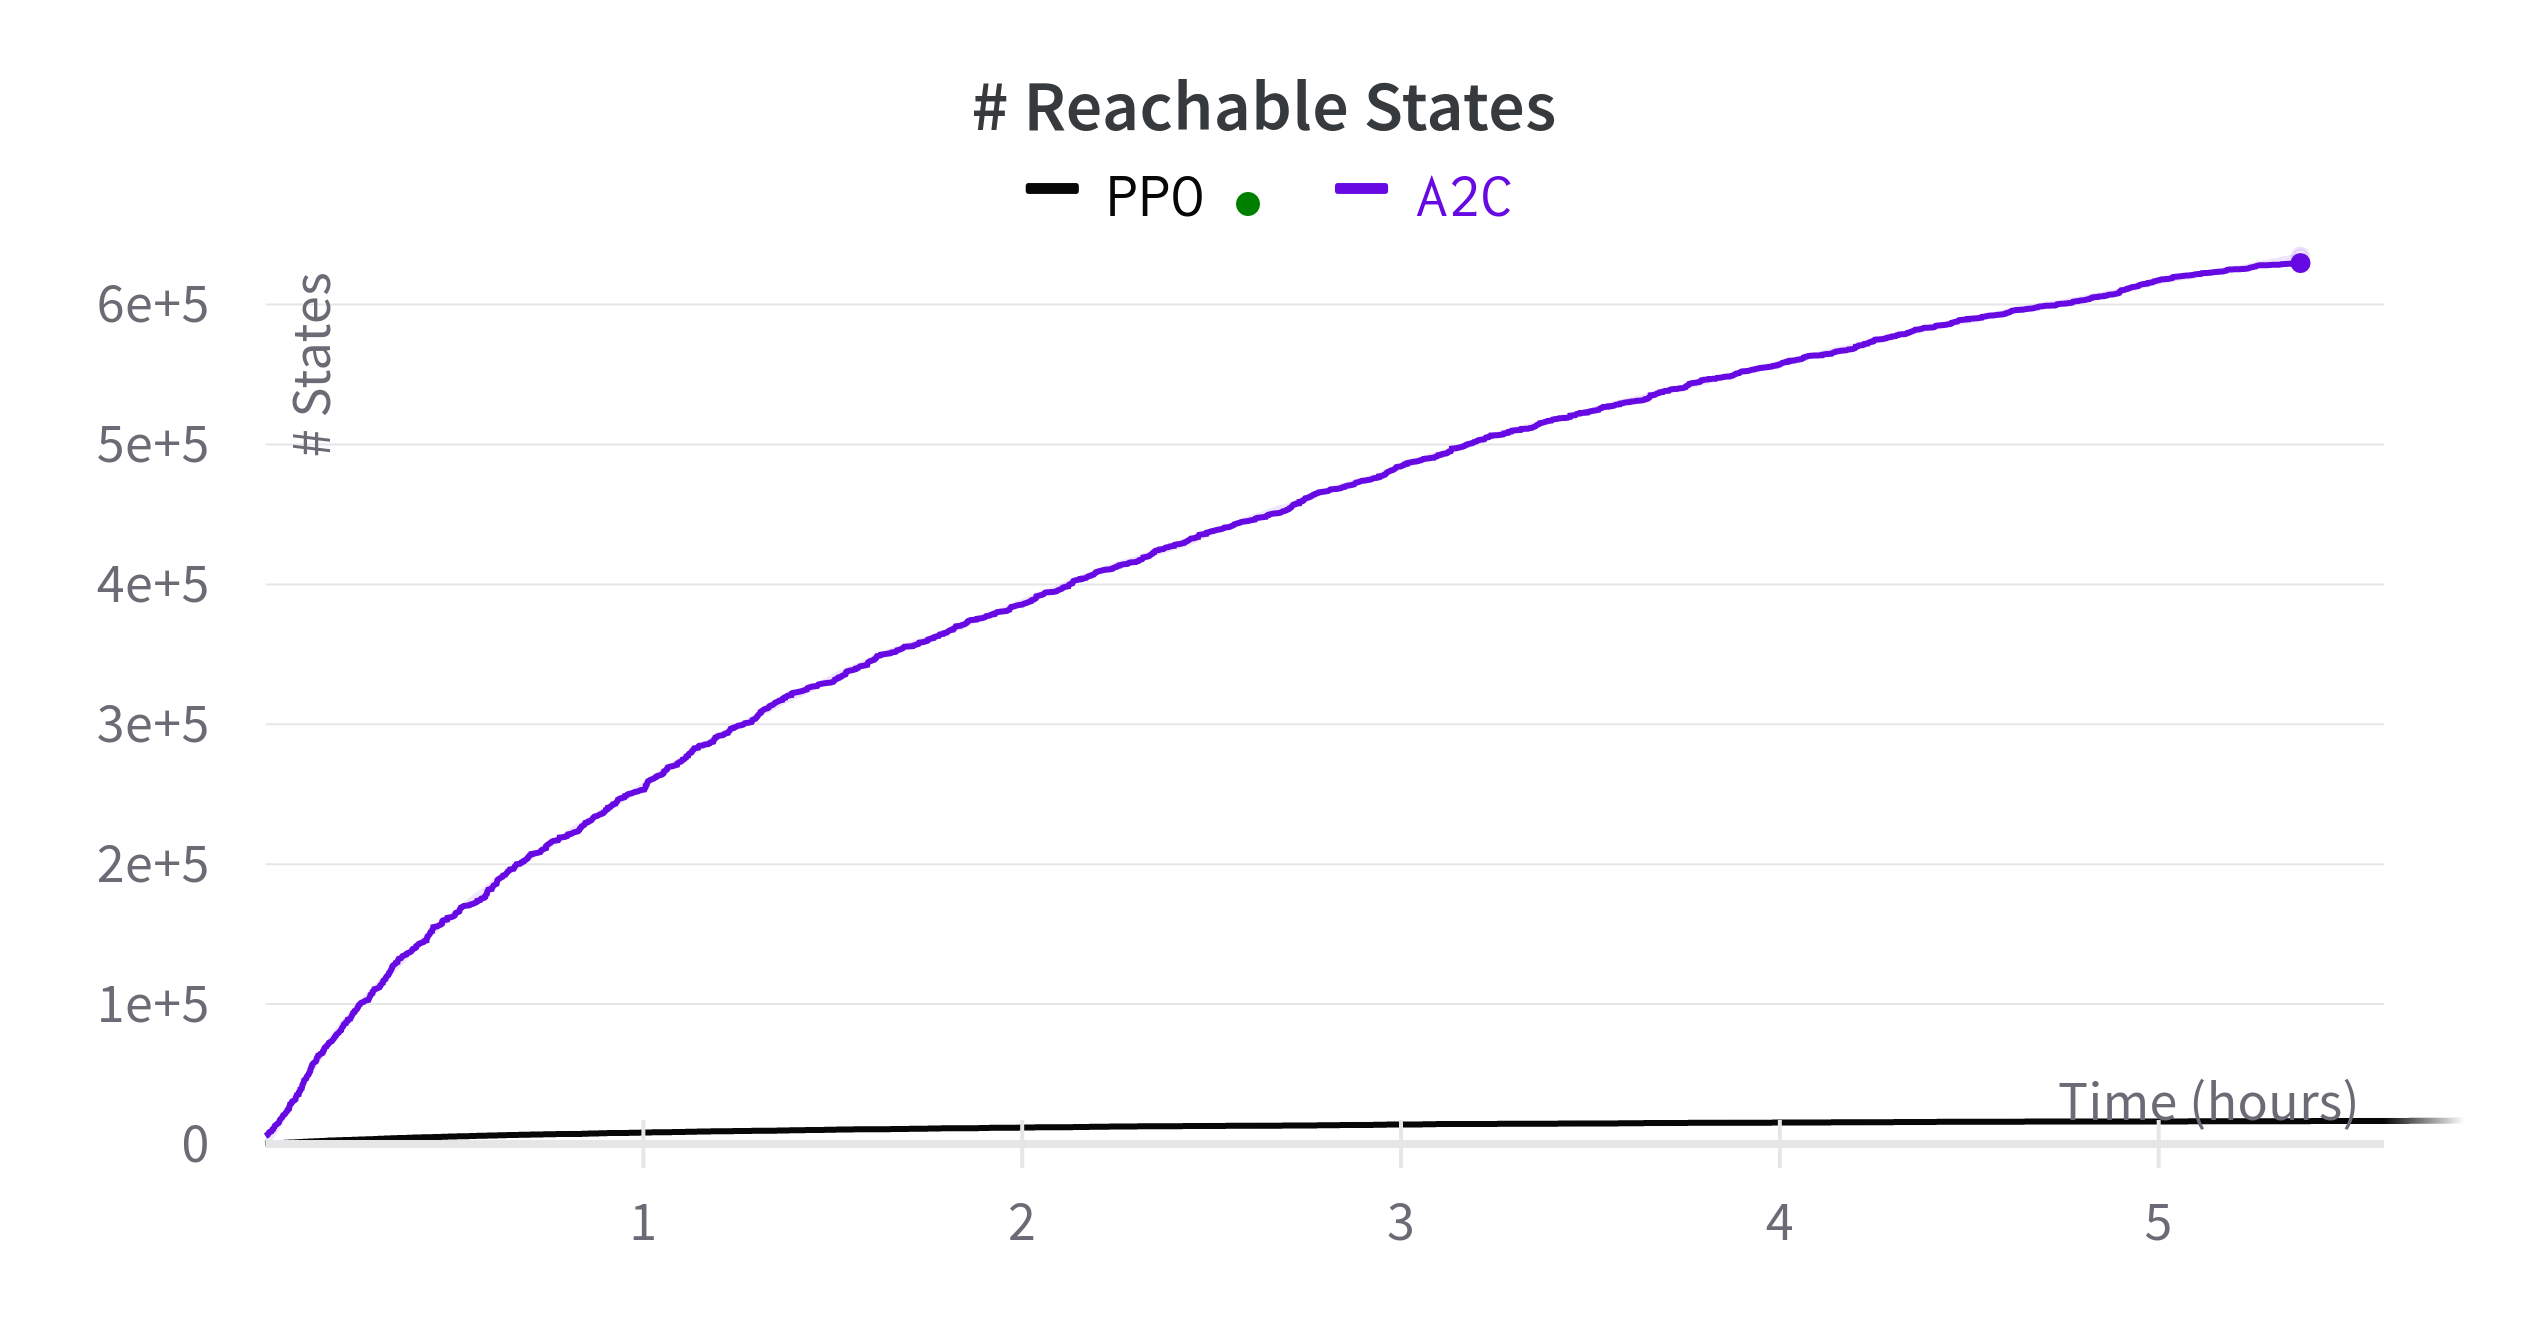
\includegraphics[width=\columnwidth]{figs/reachable_states.png}%
	\label{fig_first_case}}
\subfloat[Max state space depth observed over 25 thousand training episodes.]{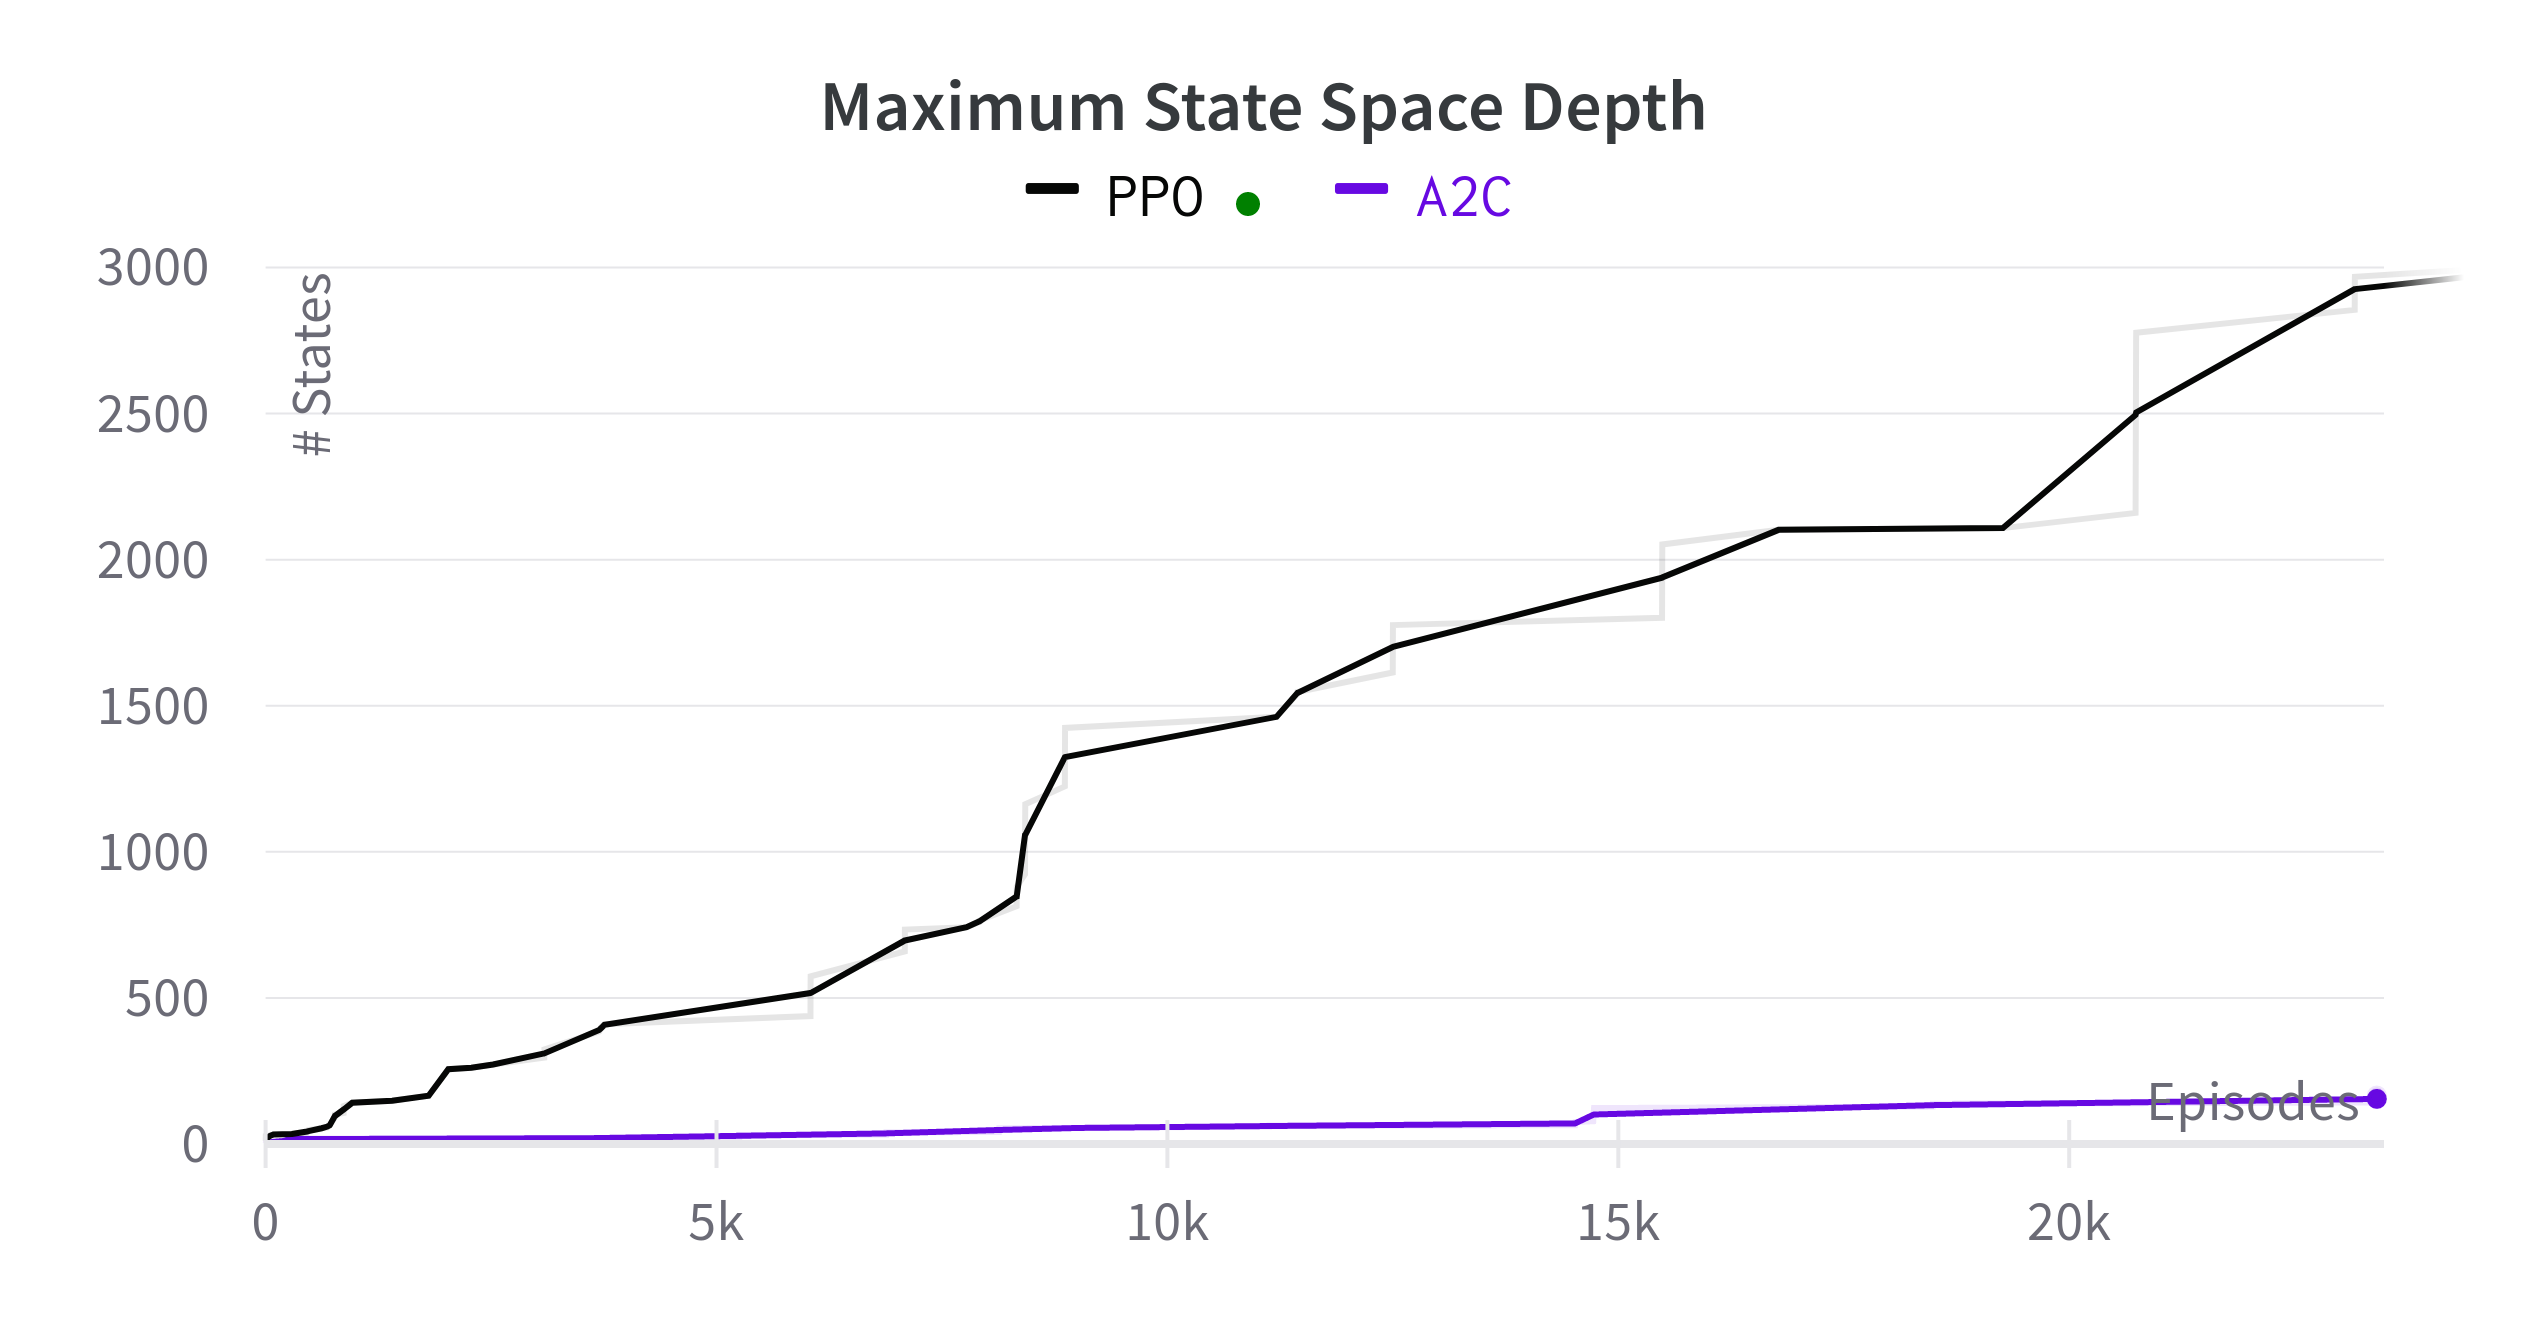
\includegraphics[width=\columnwidth]{figs/max_k.png}%
	\label{fig_second_case}}
\hfil
\subfloat[Mean policy entropy loss. The negative average entropy output by the policy network.]{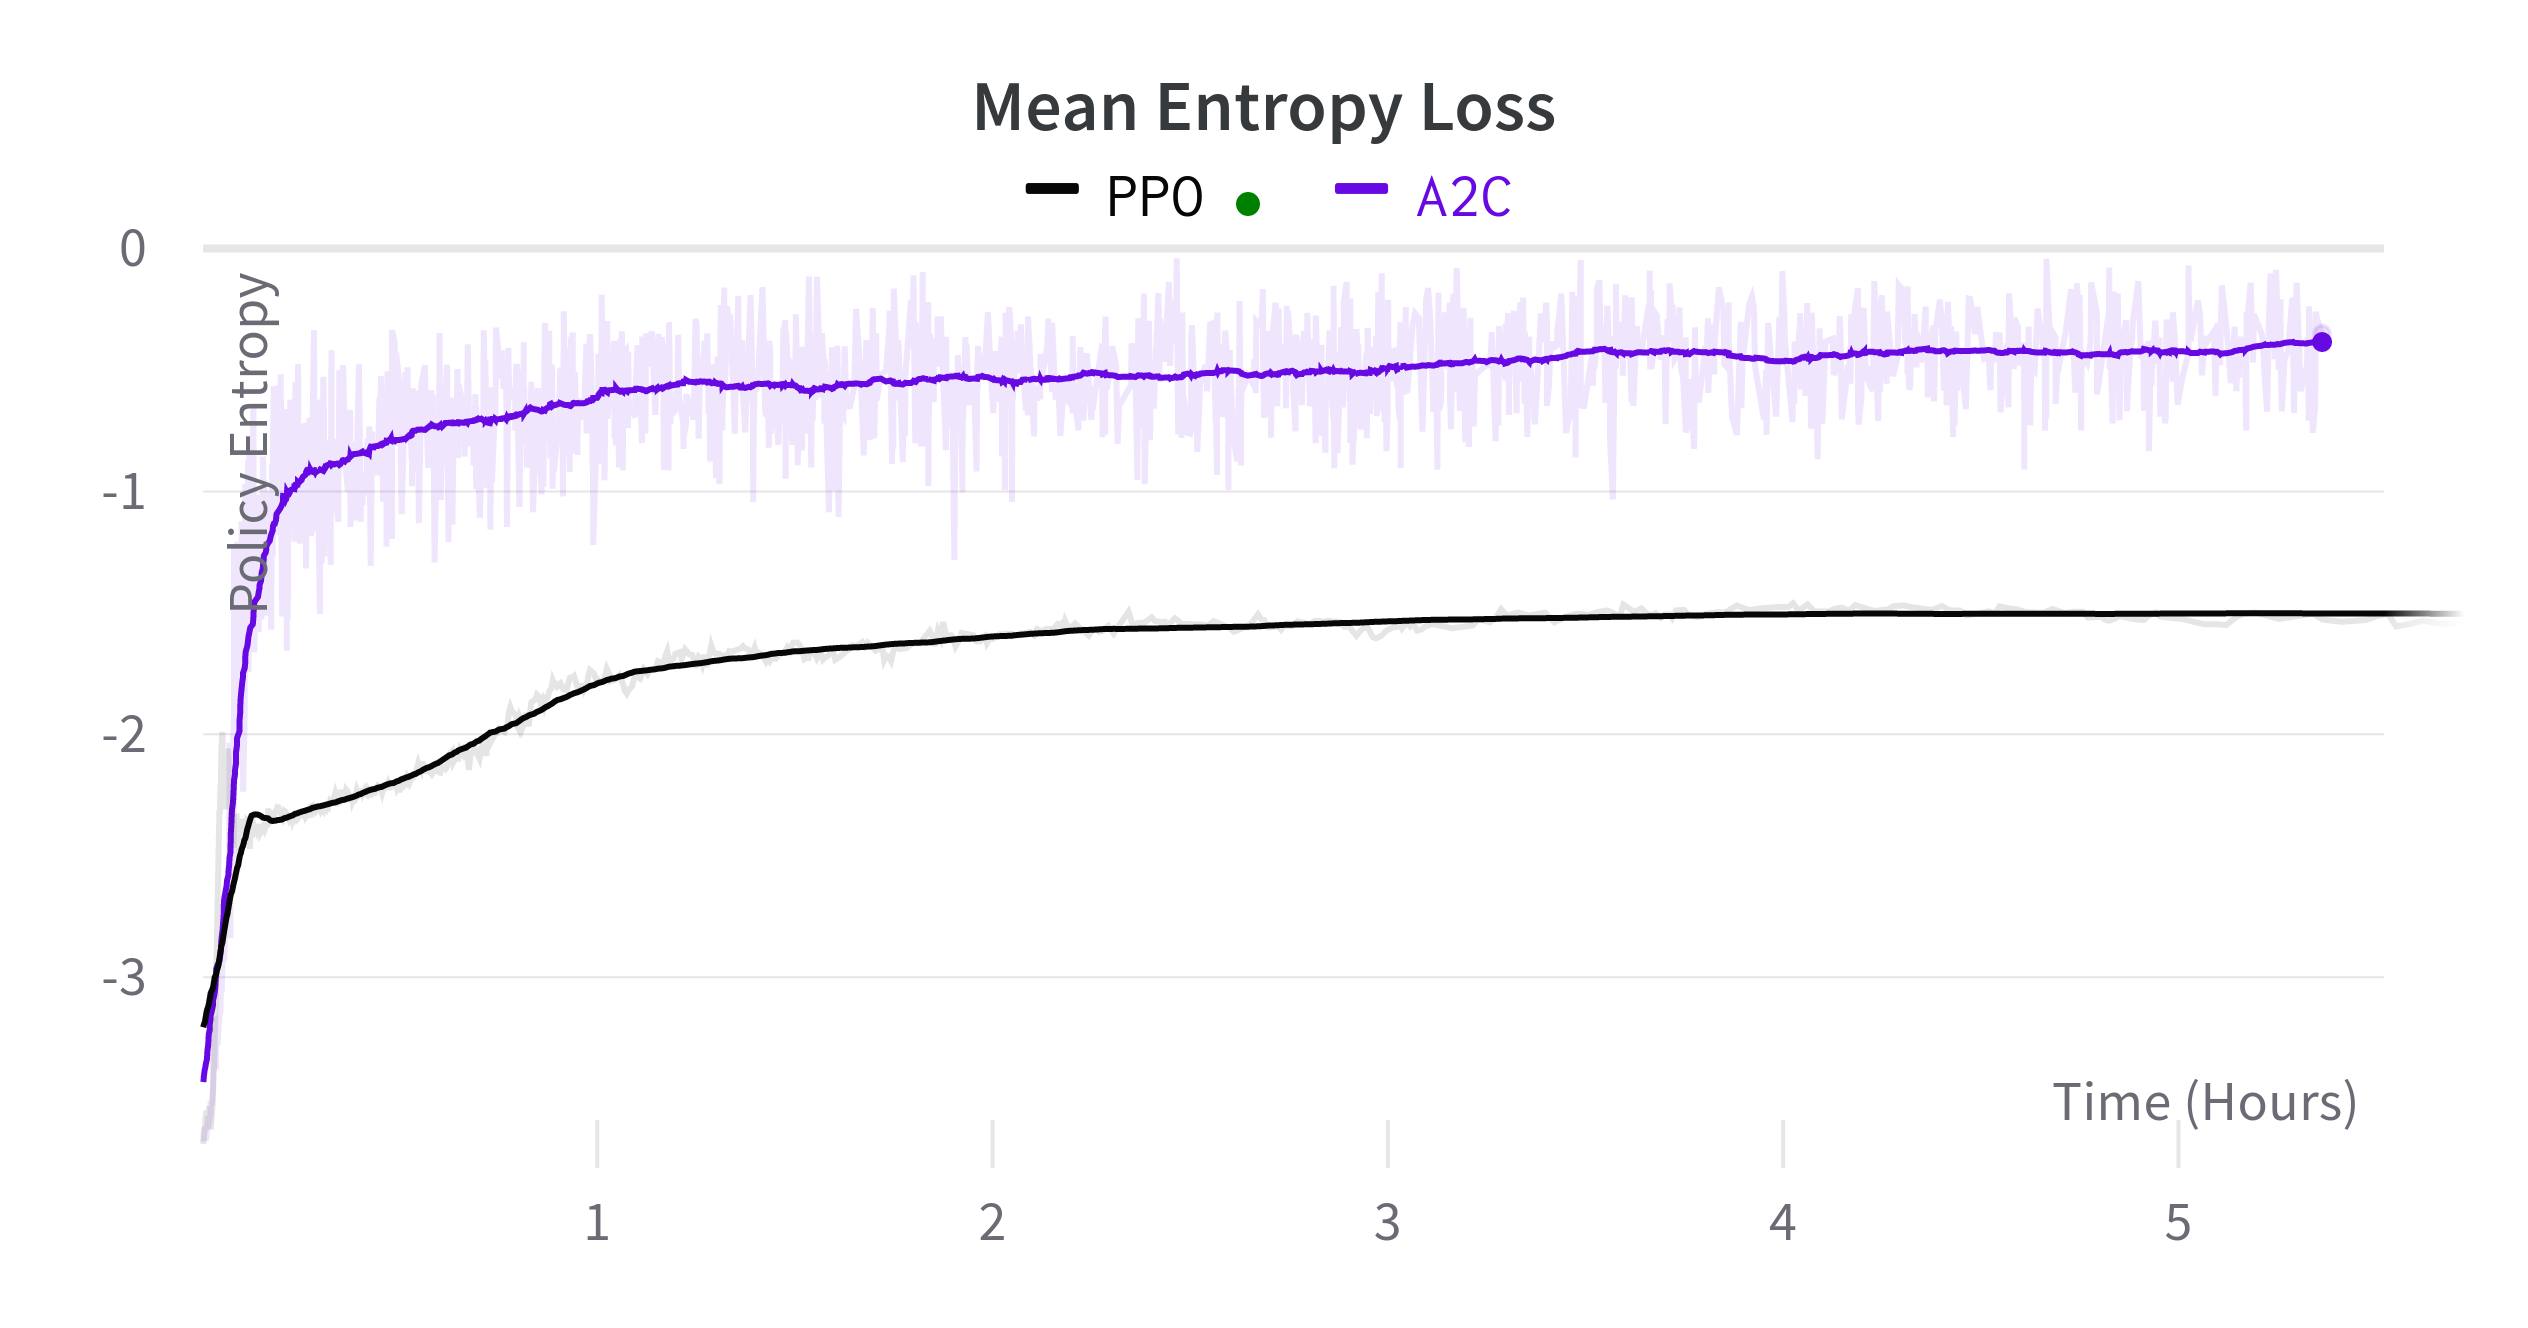
\includegraphics[width=\columnwidth]{figs/entropy.png}%
	\label{fig_first_case}}
\subfloat[Rolling average of reward for 35 thousand training episodes.]{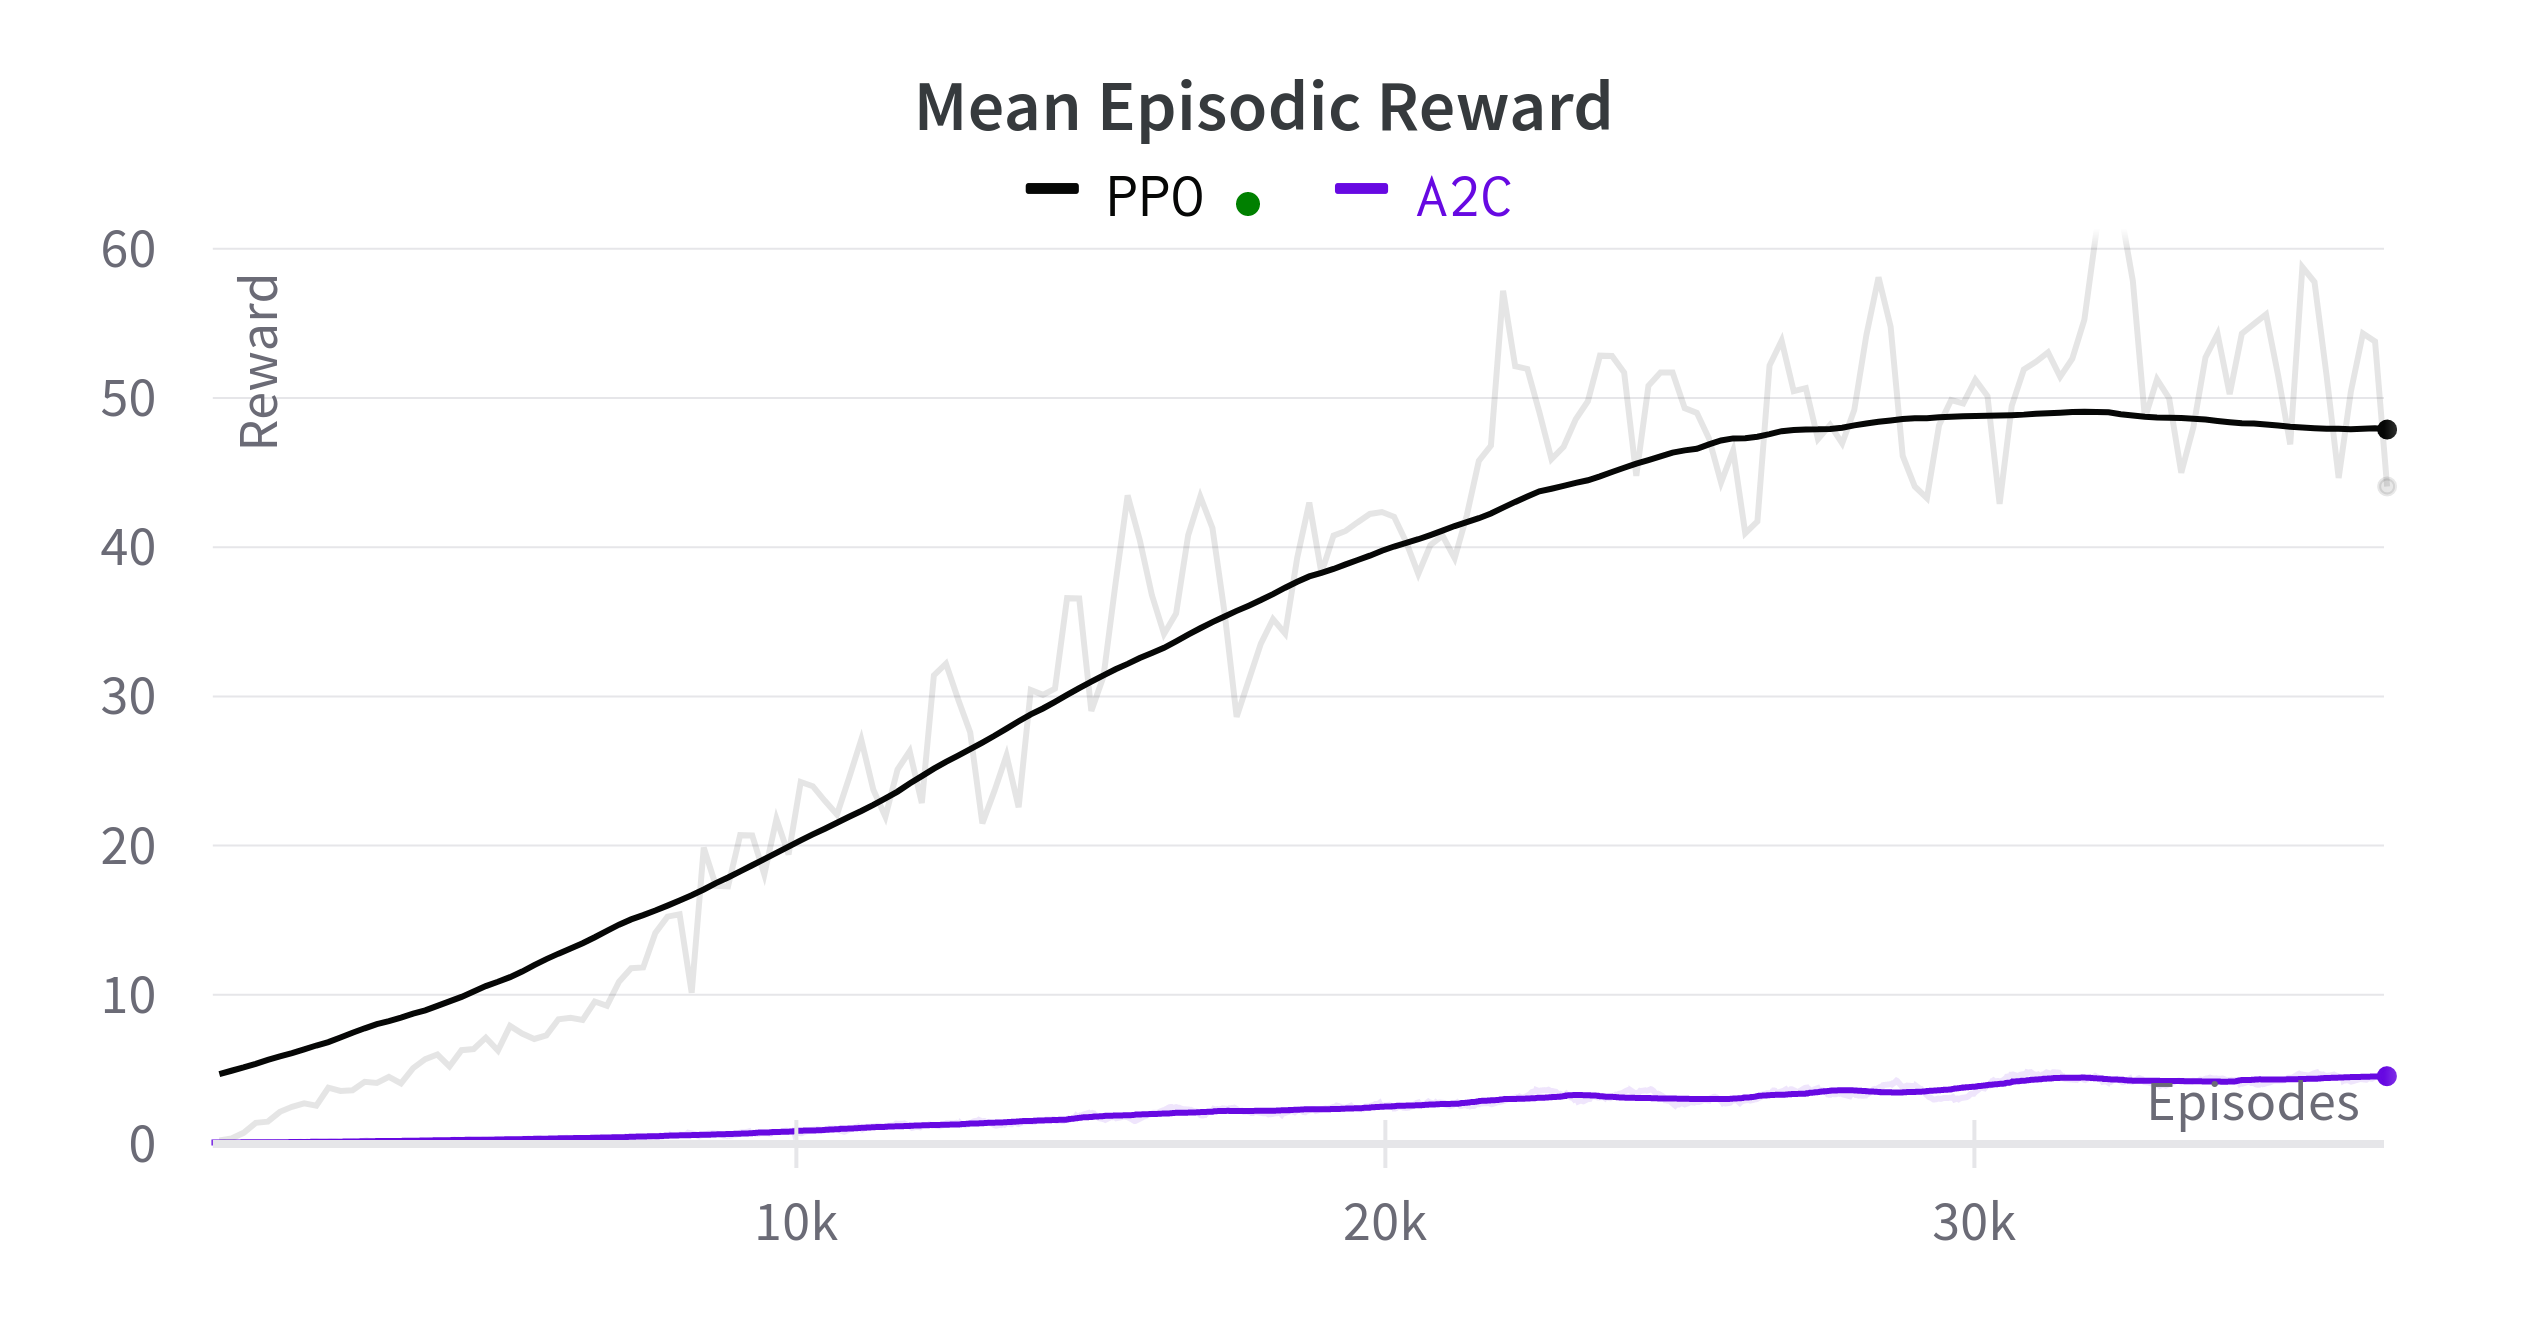
\includegraphics[width=\columnwidth]{figs/reward.png}%
	\label{fig_second_case}}
\caption{Training and evaluation metrics during application of PPO and A2C algorithms on generated state space of a theoretic size $2^{50}$.}
\label{fig:performance}
\end{figure*}
 
Advantage actor critic methods seem to perform better in terms of coverage, particularly  distributed variants. The multi agent nature paired with no update clipping may allow for greater exploration at the cost of training stability. Having observed the best coverage performance from A3C, we select a number of ladder programs to compare single agent algorithms, namely A2C and PPO, in terms of their training behaviour and evaluation performance. Having designed our reward function as one of continued state novelty we expected PPO to outperform A2C, covering a greater proportion of states after A2C performance either plateaus or collapses.


Figure~\ref{fig:performance}(a) shows the number of reachable state discovered by the agent during the first 5 hours of training on a ladder program with 19 additional rungs. A2C increases state coverage significantly faster than PPO but considering Figure~\ref{fig:performance}(b), struggles to learn which transitions reveal the max state depth within its discovered subregion.

Again, Figure~\ref{fig:performance}(b) demonstrates PPO optimises better to the actual reward objective, maximising exploration of state-action pairs for the explored subregion while slowly increasing state coverage. The surrogate clipped objective used during the gradient update may contribute to how agents introduce new states by steadily exploring uncertain state-action pairs. Figure~\ref{fig:performance}(c) may also suggest this, in that we observe the mean entropy loss for PPO is significantly more stable than that of A2C, indicating the policy under PPO maintains higher levels of uncertainty. Conversely, A2C mean entropy loss appears to converge toward 0, indicating its prediction are more certain despite very poor performance in terms of the actual reward objective. Similarly the value function loss is more stable for PPO compared to A2C. This measures the TD error between the current value function and actual observed returns.

Model performance across all learning algorithms appears sensitive to network update frequency and experience accumulation during rollout, prior to each update. This is certainly a property to be conscious of as it may translate interlocking programs, making this parameter dependent on the state space structure, where the total number of reachable states or longest acyclic path is unknown to us. In future we would like to trial this set of algorithms, as well as some hybrid approaches~\cite{haarnoja2018soft}, using a modified reward function based on global state coverage or uncertainty maximisation.

% An example of a floating figure using the graphicx package.
% Note that \label must occur AFTER (or within) \caption.
% For figures, \caption should occur after the \includegraphics.
% Note that IEEEtran v1.7 and later has special internal code that
% is designed to preserve the operation of \label within \caption
% even when the captionsoff option is in effect. However, because
% of issues like this, it may be the safest practice to put all your
% \label just after \caption rather than within \caption{}.
%
% Reminder: the "draftcls" or "draftclsnofoot", not "draft", class
% option should be used if it is desired that the figures are to be
% displayed while in draft mode.
%
%\begin{figure}[!t]
%\centering
%\includegraphics[width=2.5in]{myfigure}
% where an .eps filename suffix will be assumed under latex, 
% and a .pdf suffix will be assumed for pdflatex; or what has been declared
% via \DeclareGraphicsExtensions.
%\caption{Simulation results for the network.}
%\label{fig_sim}
%\end{figure}

% Note that the IEEE typically puts floats only at the top, even when this
% results in a large percentage of a column being occupied by floats.


% An example of a double column floating figure using two subfigures.
% (The subfig.sty package must be loaded for this to work.)
% The subfigure \label commands are set within each subfloat command,
% and the \label for the overall figure must come after \caption.
% \hfil is used as a separator to get equal spacing.
% Watch out that the combined width of all the subfigures on a 
% line do not exceed the text width or a line break will occur.
%

%
% Note that often IEEE papers with subfigures do not employ subfigure
% captions (using the optional argument to \subfloat[]), but instead will
% reference/describe all of them (a), (b), etc., within the main caption.
% Be aware that for subfig.sty to generate the (a), (b), etc., subfigure
% labels, the optional argument to \subfloat must be present. If a
% subcaption is not desired, just leave its contents blank,
% e.g., \subfloat[].


% An example of a floating table. Note that, for IEEE style tables, the
% \caption command should come BEFORE the table and, given that table
% captions serve much like titles, are usually capitalized except for words
% such as a, an, and, as, at, but, by, for, in, nor, of, on, or, the, to
% and up, which are usually not capitalized unless they are the first or
% last word of the caption. Table text will default to \footnotesize as
% the IEEE normally uses this smaller font for tables.
% The \label must come after \caption as always.
%
%\begin{table}[!t]
%% increase table row spacing, adjust to taste
%\renewcommand{\arraystretch}{1.3}
% if using array.sty, it might be a good idea to tweak the value of
% \extrarowheight as needed to properly center the text within the cells
%\caption{An Example of a Table}
%\label{table_example}
%\centering
%% Some packages, such as MDW tools, offer better commands for making tables
%% than the plain LaTeX2e tabular which is used here.
%\begin{tabular}{|c||c|}
%\hline
%One & Two\\
%\hline
%Three & Four\\
%\hline
%\end{tabular}
%\end{table}


% Note that the IEEE does not put floats in the very first column
% - or typically anywhere on the first page for that matter. Also,
% in-text middle ("here") positioning is typically not used, but it
% is allowed and encouraged for Computer Society conferences (but
% not Computer Society journals). Most IEEE journals/conferences use
% top floats exclusively. 
% Note that, LaTeX2e, unlike IEEE journals/conferences, places
% footnotes above bottom floats. This can be corrected via the
% \fnbelowfloat command of the stfloats package.


\section{Conclusion \& Future Work } 
In this work we have taken first steps towards using machine learning to generate invariants by providing a first formal mapping of interlocking based state spaces to a reinforcement learning (RL) environment. In addition, we have applied asynchronous and trust region deep reinforcement learning methods to programtically generated state spaces and analysed their ability in terms of state coverage and state space depth. Our findings highlight that RL approaches can be succesfully rewarded to explore a large percentage of a given state space in terms of state coverage, however that incentivising depth based exploration is more challenging. As any machine learning approach to finding invariants will likely need to explore such a state space these results show the credability of such an appraoch. In our subsequent works we envisage the current learning framework to serve as a means of dataset generation, from which patterns or sequences of can be mined from agent trajectories.

In light of our findings, we also aim to improve several aspects of our approach, predominantly concerning learning stability, sample efficiency and training speed. The low dimensionality of our state space representation may allow us to introduce count-based exploration models to dampen the reward issued for repeated observations~\cite{ostrovski2017countbased}. Intrinsic motivation has also demonstrated success in shaping rewards to boost environment exploration~\cite{houthooft2017vime}. Such further tuning of our reward scheme may also lead to improved coverage performance using PPO, where the learning objective may be less complex than one pursuing state space depth.

Applying modified algorithms such as IMPALA~\cite{espeholt2018impala} could improve both the sample efficiency over our A3C implementation and increase model capacity for deeper network architectures and robustness against hyperparameter adjustments. The adoption of a Long Short-Term Memory model (LSTM) could potentially improve performance by predicting candidate state sequences at discrete time steps, adding some temporality to the learned features.
% conference papers do not normally have an appendix

% use section* for acknowledgment
\ifCLASSOPTIONcompsoc
  % The Computer Society usually uses the plural form
  \section*{Acknowledgments}
\else
  % regular IEEE prefers the singular form
  \section*{Acknowledgment}
\fi
We thank Tom Werner and Andrew Lawrence at Siemens Mobility UK \& EPSRC for their support in these works.
% trigger a \newpage just before the given reference
% number - used to balance the columns on the last page
% adjust value as needed - may need to be readjusted if
% the document is modified later
%\IEEEtriggeratref{8}
% The "triggered" command can be changed if desired:
%\IEEEtriggercmd{\enlargethispage{-5in}}

% references section

% can use a bibliography generated by BibTeX as a .bbl file
% BibTeX documentation can be easily obtained at:
% http://mirror.ctan.org/biblio/bibtex/contrib/doc/
% The IEEEtran BibTeX style support page is at:
% http://www.michaelshell.org/tex/ieeetran/bibtex/
\bibliographystyle{IEEEtran}
% argument is your BibTeX string definitions and bibliography database(s)
\bibliography{bibliography}
%
% <OR> manually copy in the resultant .bbl file
% set second argument of \begin to the number of references
% (used to reserve space for the reference number labels box)




% that's all folks
\end{document}


